
\documentclass[a4paper,fleqn]{cas-sc}
\usepackage[authoryear,longnamesfirst]{natbib}
\usepackage{booktabs}
\usepackage{amsmath}
\usepackage{amssymb}
\usepackage{bm}
\usepackage{hyperref}

\begin{document}
\let\WriteBookmarks\relax
\def\floatpagepagefraction{1}
\def\textpagefraction{.001}

\title{Elephant Attention and North American Seagull Memory: A Unified Method for Long-Horizon Multi-Agent LLM Systems}
\date{}

\maketitle

\begin{abstract}
Large language model agents are increasingly expected to solve long-horizon tasks that require tool use, delegation, retrieval, and cross-session continuity. However, simply extending context windows or adding more agents does not resolve the underlying methodological problem: long-running multi-agent systems must jointly decide what to attend to, what to retain, what to compress, and how to preserve behavioral continuity under bounded prompt budgets. Existing studies usually address these issues in isolation, focusing on agent decomposition, long-context modeling, retrieval augmentation, or memory modules separately.

This paper proposes the \emph{Elephant-Seagull Framework}, a unified method for long-horizon multi-agent LLM systems. The framework is organized around four coordinated mechanisms: \emph{Elephant Attention}, a system-level salience policy that prioritizes validated, reusable, and socially significant context; \emph{North American Seagull Memory}, a migratory long-term memory mechanism that governs when memory should leave local execution scope, persist across runs, and return under future relevance; \emph{Long-Horizon Attention}, which maintains execution continuity through windows, summaries, snapshots, and artifact rollups; and \emph{Context Compression}, which formulates prompt construction as a budget-constrained selection problem over typed context segments.

The method further closes the loop with \emph{MGCM} (Matriarch-Governed Collective Memory) and \emph{event-centric observability}, linking local memory, candidate shared notes, collective promotion, and todo projection into a single governance process. In this formulation, observability is not treated as a peripheral logging facility, but as part of the method itself because it provides structured evidence for memory promotion, debugging, and progress-state reconstruction.

This manuscript is written as a pure method paper. Rather than claiming completed benchmark superiority without evidence, it specifies a rigorous evaluation program for validating long-horizon performance, memory reuse, budget robustness, and interpretability. The contribution is therefore a unified research framework and an executable experimental design for studying long-horizon multi-agent LLM systems under realistic coordination and context constraints.
\end{abstract}

\noindent\textbf{Keywords:} large language model agents; multi-agent systems; Elephant Attention; North American Seagull Memory; long-horizon reasoning; context compression; MGCM; event-centric observability.

\section{Introduction}

Large language models are rapidly evolving from single-turn generators into autonomous systems that plan, retrieve, invoke tools, coordinate with external software, and maintain task state over extended horizons. Survey evidence suggests that the practical capability of such systems no longer depends only on the base model, but on the surrounding agentic stack that controls reasoning, memory, environment interaction, and self-monitoring \citep{wang2024survey}. This shift becomes even more pronounced when the workload exceeds a single prompt-response cycle. Long-form research, coding, analysis, or multi-stage execution requires a system to survive many decisions, tool calls, subtask handoffs, and delayed feedback. In such settings, single-agent prompting and naive long-context accumulation become increasingly brittle.

The core difficulty is not merely one of scale, but one of coupled governance. Long-horizon multi-agent systems face at least four interdependent challenges. First, collaboration introduces coordination pressure: the system must decide which agent should act, what context should be handed off, and how specialist outputs should influence collective behavior. Second, long-term operation introduces memory pressure: the system must decide what should remain ephemeral, what should be promoted to shared memory, and what deserves durable persistence across runs. Third, bounded prompt budgets introduce compression pressure: candidate context almost always exceeds usable prompt capacity. Fourth, extended execution introduces observability pressure: without structured traces, it becomes difficult to diagnose failure, estimate costs, or even reconstruct what happened during a run.

Existing research addresses important parts of this problem but seldom unifies them. Work on LLM-based autonomous agents emphasizes planning, tool use, and feedback loops \citep{wang2024survey, yao2023react, shinn2023reflexion}. Work on LLM-based multi-agent systems studies role specialization, decomposition, and collective behavior \citep{jimenezromero2025mas, wooldridge2009}. Work on long-context modeling focuses on extending usable windows and positional robustness \citep{li2024sbarope}. Retrieval and memory work improves access to external knowledge and historical evidence \citep{lewis2020rag}. Yet these directions often remain modular add-ons. The literature still lacks a unified method that treats collaborative salience, long-term migratory memory, long-horizon continuity, and budgeted context compression as parts of the same governing framework.

This paper proposes such a framework. We introduce \emph{Elephant Attention} as a system-level policy for prioritizing validated and socially significant context during a run, and \emph{North American Seagull Memory} as a complementary mechanism for migrating durable memory across runs and returning it when future conditions warrant reuse. We then place these ideas inside a broader framework that includes \emph{Long-Horizon Attention} for maintaining continuity over long trajectories and \emph{Context Compression} for budget-constrained prompt construction. To make the full loop explicit, we integrate these mechanisms with MGCM and an \emph{event-centric observability} layer that projects execution traces into interpretable todo states and structured evidence for memory governance.

The contributions of this paper are as follows.
\begin{enumerate}
\item We propose \textbf{Elephant Attention}, a system-level salience policy that reallocates attention from pure recency toward validated, reusable, and socially significant context in multi-agent LLM execution.
\item We propose \textbf{North American Seagull Memory}, a migratory long-term memory mechanism that formalizes memory migration, persistence, and return across runs and threads instead of treating memory as simple transcript accumulation.
\item We present a \textbf{unified long-horizon method framework} that combines Elephant Attention, North American Seagull Memory, Long-Horizon Attention, and Context Compression under a single budget-aware formulation.
\item We define an \textbf{event-centric observability and evaluation framework} that links MGCM, run events, and todo projection to support interpretable analysis, debugging, and future empirical validation.
\end{enumerate}

\section{Related Work}

\subsection{LLM Autonomous Agents}

LLM autonomous agents are typically framed as systems that interleave reasoning, action, and environment feedback rather than operating as one-shot text generators. Survey work has emphasized components such as planning, memory, action modules, and self-reflection \citep{wang2024survey}. ReAct demonstrated the value of explicitly coupling reasoning traces with tool-oriented action \citep{yao2023react}, while Reflexion introduced verbal self-improvement from execution feedback \citep{shinn2023reflexion}. These works are foundational because they establish that performance depends on structured execution loops. However, they are primarily centered on single-agent behavior, and they do not fully specify how collaborative salience, cross-run memory migration, and budget-aware observability should be jointly governed in long-horizon multi-agent settings.

\subsection{LLM-Based Multi-Agent Systems}

LLM-based multi-agent systems extend the agent paradigm by introducing role specialization, supervisor-worker decomposition, negotiation, and collaborative exploration. Recent surveys and application studies indicate that multi-agent architectures can improve coverage, parallelism, and problem decomposition, but can also introduce coordination cost and communication noise \citep{jimenezromero2025mas, wooldridge2009}. Most multi-agent work, however, treats coordination as a routing or role-assignment problem. Comparatively less attention has been given to the question of which context should propagate across agents, how validated knowledge should become collectively influential, and how execution traces should support both governance and interpretability.

\subsection{Long-Context and Long-Horizon Reasoning}

Extending context length has become a major research direction because many real tasks exceed the stable operating range of naive prompt accumulation. Work on rotary position embedding variants and other long-context techniques improves representational robustness under larger windows \citep{li2024sbarope}. Yet long-horizon execution is not reducible to context length alone. A system may possess a long context window and still fail because it cannot preserve procedural continuity, distinguish high-value from low-value history, or maintain a coherent compressed state over time. Our formulation therefore treats long-horizon reasoning as a runtime governance problem, not only a model-capacity problem.
\subsection{Retrieval, Memory, and Context Management}

Retrieval-augmented generation showed that external knowledge access can substantially improve knowledge-intensive tasks \citep{lewis2020rag}. More broadly, agentic systems increasingly rely on retrieval, episodic memory, workspace artifacts, and summarization to cope with scale. However, naive accumulation often increases noise, and simple retrieval does not solve the harder question of what should persist, what should be promoted, and what should return later. Our framework differs by jointly modeling in-run salience, governed promotion, migratory long-term storage, and budget-constrained compression within the same method pipeline.

\subsection{Positioning of This Work}

Relative to prior work, the proposed method makes three distinctions. First, it separates \emph{in-run salience governance} from \emph{cross-run migratory memory}, formalized as Elephant Attention versus North American Seagull Memory. Second, it treats \emph{long-horizon continuity} and \emph{context compression} as coupled optimization problems under prompt budgets rather than heuristic utilities. Third, it elevates \emph{event-centric observability} from engineering instrumentation to methodological infrastructure because structured traces enable progress projection, memory governance, and failure analysis. The result is a unified framework for long-horizon multi-agent LLM systems rather than a collection of loosely connected components.

\section{Problem Formulation}

We consider a long-horizon multi-agent LLM system that receives a user request $x$, operates within a thread state $\mathcal{H}_t$, has access to a tool set $\mathcal{T}$, a retrievable knowledge substrate $\mathcal{R}$, a set of available agents $\mathcal{A}$, and multiple memory stores. At decision step $t$, the system must construct an executable prompt context $\mathcal{C}_t$ and choose an action $a_t$ from the action space
\begin{equation}
\mathcal{U} = \mathcal{U}_{\text{reason}} \cup \mathcal{U}_{\text{tool}} \cup \mathcal{U}_{\text{retrieve}} \cup \mathcal{U}_{\text{delegate}} \cup \mathcal{U}_{\text{memory}}.
\end{equation}
Here, the action can be a direct reasoning step, a tool call, a retrieval request, a delegation event, or a memory-governance update.

The candidate context before compression is
\begin{equation}
\mathcal{X}_t = \mathcal{H}_t \cup \mathcal{M}^{\text{local}}_t \cup \mathcal{M}^{\text{collective}}_t \cup \mathcal{M}^{\text{migratory}}_t \cup \mathcal{R}_t \cup \mathcal{D}_t \cup \mathcal{S}_t,
\end{equation}
where $\mathcal{M}^{\text{local}}_t$ denotes local working memory, $\mathcal{M}^{\text{collective}}_t$ denotes governed shared memory, $\mathcal{M}^{\text{migratory}}_t$ denotes North American Seagull long-term memory candidates returned from prior runs, $\mathcal{R}_t$ denotes retrieved evidence, $\mathcal{D}_t$ denotes delegation packets and coordination metadata, and $\mathcal{S}_t$ denotes strategy instructions or structured control segments.

Prompt construction is constrained by a finite token or character budget $B_t$. Let each candidate segment $z_i \in \mathcal{X}_t$ have size $\ell_i$. The prompt builder must select a subset $\mathcal{C}_t \subseteq \mathcal{X}_t$ such that
\begin{equation}
\sum_{z_i \in \mathcal{C}_t} \ell_i \leq B_t.
\end{equation}
This turns context construction into a constrained selection problem rather than an append-only transcript problem.

Multi-agent execution additionally introduces a routing policy
\begin{equation}
\pi_{\text{route}} : (x, \mathcal{H}_t, \mathcal{X}_t) \mapsto \{(\alpha_j, \tau_j)\}_{j=1}^{m_t},
\end{equation}
where $\alpha_j \in \mathcal{A}$ is a selected agent and $\tau_j$ is a compact task packet. The system must determine not only which agent should act, but also what compacted context and memory evidence should accompany the delegation.

Memory is governed across four levels:
\begin{equation}
\mathcal{M}_t = \{\mathcal{M}^{\text{local}}_t, \mathcal{M}^{\text{candidate}}_t, \mathcal{M}^{\text{collective}}_t, \mathcal{M}^{\text{migratory}}_t\}.
\end{equation}
Local memory supports the current run; candidate memory stores unvalidated intermediate knowledge; collective memory stores validated shared knowledge; migratory memory stores persistent cross-run memory eligible for later return.

Finally, execution emits an event stream
\begin{equation}
\mathcal{E} = (e_1, e_2, \ldots, e_T),
\end{equation}
where each event contains identifiers such as run ID, thread ID, task ID, stage, and metadata. These events are not auxiliary artifacts; they are part of the formal object of study because they support both runtime observability and event-derived todo projection.

Under this formulation, the research problem is to design a unified policy family
\begin{equation}
\Pi = \{\pi_{\text{elephant}}, \pi_{\text{seagull}}, \pi_{\text{horizon}}, \pi_{\text{compress}}, \pi_{\text{mgcm}}, \pi_{\text{obs}}\}
\end{equation}
that improves long-horizon multi-agent performance, continuity, and interpretability under bounded context budgets and multi-step execution.

\section{Method}

\subsection{Overall Framework}

The proposed \emph{Elephant-Seagull Framework} is a unified runtime method for long-horizon multi-agent LLM systems. Its execution pipeline can be summarized as
\begin{equation}
x \rightarrow \text{routing} \rightarrow \text{context construction} \rightarrow \text{reasoning/delegation} \rightarrow \text{tool/retrieval execution} \rightarrow \text{memory promotion/migration} \rightarrow \text{observability projection}.
\end{equation}

Given a request $x$, the system first resolves a routing policy that decides whether the task remains single-agent, enters a workflow, or is delegated to specialist agents. It then constructs candidate context from thread history, memory layers, retrieved evidence, strategy instructions, and delegation packets. Elephant Attention and Context Compression jointly determine which segments survive under the current prompt budget. The active agent or supervisor reasons over the compressed prompt, invokes tools or retrieval when needed, and may further delegate subtasks. After execution, MGCM determines whether produced knowledge remains local, becomes a candidate shared note, or is promoted into collective memory. North American Seagull Memory then decides which high-value memories should migrate into persistent cross-run storage and under what conditions they should return in future runs. In parallel, all execution stages emit structured events that are persisted and projected into a todo view for progress reconstruction.

This formulation makes the framework method-centric rather than architecture-centric. The emphasis is not on enumerating software modules, but on specifying how context, memory, and coordination are jointly governed across time.

\subsection{Elephant Attention}

Elephant Attention is not a neural attention layer. It is a system-level salience policy that ranks candidate context according to durable importance during collaborative execution. For each candidate segment $z_i \in \mathcal{X}_t$, we define an Elephant Attention score
\begin{equation}
s_i^{\text{EA}} = \alpha \, \mathrm{Rel}(z_i, x) + \beta \, \mathrm{Val}(z_i) + \gamma \, \mathrm{Reuse}(z_i) + \delta \, \mathrm{Out}(z_i) - \lambda \, \mathrm{Red}(z_i),
\end{equation}
where $\mathrm{Rel}$ measures task relevance, $\mathrm{Val}$ measures validation support, $\mathrm{Reuse}$ measures prior reuse across runs or agents, $\mathrm{Out}$ measures association with successful outcomes, and $\mathrm{Red}$ penalizes redundancy.

The governing bias of Elephant Attention is
\begin{equation}
\beta + \gamma + \delta > \alpha_{\text{recency}},
\end{equation}
meaning that validated, reusable, and outcome-supported context can outrank merely recent context. This differs from recency-dominant prompt assembly, which tends to overvalue fresh but unstable interaction history.

In practice, Elephant Attention solves a collaboration-specific problem: \emph{what should remain influential when many agents, tools, and sub-results compete for limited prompt budget?} The mechanism is especially important when specialist outputs and previously validated rules should continue to shape decisions even after the local conversation has advanced.

\subsection{North American Seagull Memory}

North American Seagull Memory governs long-term migratory memory. Its purpose is different from Elephant Attention. Elephant Attention prioritizes which context matters \emph{during the current run}, whereas North American Seagull Memory decides which memory should \emph{leave the current run}, persist durably, and return later under suitable conditions.

For a memory candidate $m$, we define a migration score
\begin{equation}
\mu(m) = \rho_1 \, \mathrm{Val}(m) + \rho_2 \, \mathrm{Reuse}(m) + \rho_3 \, \mathrm{Out}(m) + \rho_4 \, \mathrm{Gen}(m) - \rho_5 \, \mathrm{Noise}(m),
\end{equation}
where $\mathrm{Gen}$ measures cross-task generality and $\mathrm{Noise}$ penalizes local or low-confidence artifacts. Migration occurs if
\begin{equation}
\mu(m) \geq \theta_{\text{mig}}.
\end{equation}
When a new run begins, migratory memory does not return wholesale. Instead, each stored item receives a return score
\begin{equation}
r(m, x, \mathcal{H}_t) = \kappa_1 \, \mathrm{Match}(m, x) + \kappa_2 \, \mathrm{Thread}(m, \mathcal{H}_t) + \kappa_3 \, \mathrm{Reuse}(m) - \kappa_4 \, \mathrm{Stale}(m),
\end{equation}
and is reintroduced only if
\begin{equation}
r(m, x, \mathcal{H}_t) \geq \theta_{\text{return}}.
\end{equation}

This yields a migratory memory model: memory is promoted out of local execution when it is sufficiently validated and general, then returns only when future tasks, threads, or execution states make it useful again. The key claim is that durable memory should behave more like selective migration than passive accumulation.

\subsection{Long-Horizon Attention}

Long-Horizon Attention maintains execution continuity across long trajectories. It is not equivalent to long-term memory. Long-term memory governs what persists across runs, whereas Long-Horizon Attention governs how the \emph{current run} preserves state across many steps without replaying the entire past.

At step $t$, the maintained long-horizon state is
\begin{equation}
\mathcal{L}_t = \mathcal{W}_t \cup \Sigma_t \cup \mathcal{P}_t \cup \mathcal{A}_t,
\end{equation}
where $\mathcal{W}_t$ is a recent window, $\Sigma_t$ is a compact summary of older interaction, $\mathcal{P}_t$ is a structured snapshot of procedural state, and $\mathcal{A}_t$ is an artifact rollup capturing persistent outputs such as notes, plans, or partial deliverables.

The summary and snapshot components are refreshed periodically:
\begin{equation}
\Sigma_{t+1} =
\begin{cases}
g(\mathcal{H}_{0:t}) & \text{if } t \bmod k_{\Sigma} = 0, \\
\Sigma_t & \text{otherwise,}
\end{cases}
\end{equation}
\begin{equation}
\mathcal{P}_{t+1} =
\begin{cases}
\phi(\text{state}_t) & \text{if } t \bmod k_{P} = 0, \\
\mathcal{P}_t & \text{otherwise.}
\end{cases}
\end{equation}
Artifact rollups are similarly updated every $k_A$ steps or after major tool/retrieval milestones.

The role of Long-Horizon Attention is to preserve trajectory-level coherence. It maintains what the system is trying to do, what has already been done, what artifacts matter, and where execution currently stands, even when the raw transcript is too large to keep in full.

\subsection{Context Compression}

Context Compression translates heterogeneous candidate context into a budgeted optimization problem. Let each segment $z_i$ have type $t_i$, size $\ell_i$, Elephant Attention score $s_i^{\text{EA}}$, and stage-aware weight $\omega(t_i, \sigma_t)$ determined by the current execution stage $\sigma_t$. We define the effective segment utility as
\begin{equation}
u_i = \omega(t_i, \sigma_t) \cdot s_i^{\text{EA}} - \xi \, \mathrm{Red}(z_i),
\end{equation}
where $\mathrm{Red}(z_i)$ captures redundancy inhibition.

Prompt construction is then written as
\begin{align}
\max_{\bm{b}} \quad & \sum_{i=1}^{n} b_i u_i \\
\text{s.t.} \quad & \sum_{i=1}^{n} b_i \ell_i \leq B_t, \\
& b_i \in \{0,1\}.
\end{align}

This selection operates over typed segments rather than raw text blocks. The types may include conversation history, memory capsules, retrieved evidence, delegation packets, task instructions, summaries, and artifacts. Stage-aware weighting allows the system to prefer different segment classes at different phases of execution; for example, delegation packets may receive higher weight during routing, while tool observations may receive higher weight during post-tool reasoning.

Context Compression therefore differs from simple truncation in three ways. First, it uses typed segments rather than position-only heuristics. Second, it uses stage-aware weighting rather than a universal fixed rule. Third, it explicitly inhibits redundancy so that repeated evidence does not crowd out higher-value context under the same budget.

\subsection{Memory Governance and Event-Centric Progress Projection}

The framework closes the loop by coupling memory governance with event-centric observability. MGCM organizes memory into local memory, candidate shared notes, collective memory, and migratory long-term memory. For a candidate memory item $m$, we define a promotion score
\begin{equation}
p(m) = \eta_1 \, \mathrm{Rel}(m) + \eta_2 \, \mathrm{Evi}(m) + \eta_3 \, \mathrm{Reuse}(m) + \eta_4 \, \mathrm{Out}(m) + \eta_5 \, \mathrm{Coll}(m),
\end{equation}
where $\mathrm{Evi}$ denotes evidence support and $\mathrm{Coll}$ denotes collective reinforcement. Promotion into governed collective memory occurs when
\begin{equation}
p(m) \geq \theta_{\text{promote}},
\end{equation}
while promotion into migratory long-term memory additionally requires
\begin{equation}
\lambda_1 p(m) + \lambda_2 \mu(m) \geq \theta_{\text{long}}.
\end{equation}

Execution simultaneously emits an event stream
\begin{equation}
\mathcal{E} = (e_1, e_2, \ldots, e_T),
\end{equation}
including run start, task creation, reasoning stages, tool calls, retrieval completion, delegation, human feedback, and run completion. We define a todo projection operator
\begin{equation}
\Psi : \mathcal{E} \rightarrow \mathcal{Q},
\end{equation}
where $\mathcal{Q}$ is the run-level progress state. Each todo item $q_k \in \mathcal{Q}$ is updated incrementally:
\begin{equation}
q_k^{(t+1)} = \Psi(q_k^{(t)}, e_{t+1}).
\end{equation}

This event-centric view serves two methodological roles. First, it provides structured evidence for memory governance, since promotion decisions can depend on validated traces, reuse statistics, and outcomes. Second, it provides interpretable progress reconstruction for long-horizon runs. In this sense, event-centric observability is part of the reasoning-and-memory loop rather than an external logging utility.

\section{Experimental Design}

\subsection{Research Questions}

The proposed method should be evaluated through the following research questions.
\begin{enumerate}
\item \textbf{RQ1:} Does the Elephant-Seagull Framework outperform single-agent and ordinary multi-agent baselines on long-horizon complex tasks?
\item \textbf{RQ2:} Does Elephant Attention improve context selection quality and collaboration stability relative to recency-dominant context assembly?
\item \textbf{RQ3:} Does North American Seagull Memory improve cross-run and cross-thread long-term memory reuse compared with naive memory accumulation?
\item \textbf{RQ4:} Do Long-Horizon Attention and Context Compression preserve task performance under constrained prompt budgets?
\item \textbf{RQ5:} Does event-centric observability with todo projection improve interpretability, debugging quality, and trace completeness compared with plain logs?
\end{enumerate}

\subsection{Tasks and Benchmarks}

This paper does not report fabricated benchmark results. Instead, it specifies a benchmark-first evaluation suite that should be implemented next. Rather than relying on ad hoc demo tasks, each research question is tied to named public benchmark families and then instantiated in the current codebase through benchmark-aligned local slices for reproducible dry runs.
\begin{itemize}
\item \textbf{RQ1} should anchor on \textbf{GAIA} for tool-augmented long-horizon task execution, with \textbf{HotpotQA} and \textbf{MuSiQue} serving as additional multi-hop reasoning and compositional reasoning references.
\item \textbf{RQ2} should anchor on distractor-heavy subsets inspired by \textbf{HotpotQA} and \textbf{MuSiQue}, because the main question is whether Elephant Attention preserves validated evidence under noisy context competition.
\item \textbf{RQ3} should anchor on \textbf{LoCoMo} and \textbf{LongMemEval}, which are better aligned with the claim that North American Seagull Memory improves cross-run and cross-thread memory return.
\item \textbf{RQ4} should anchor on \textbf{LongBench} and \textbf{InfiniteBench}, because the main hypothesis concerns performance degradation under constrained prompt budgets and long-context stress.
\item \textbf{RQ5} currently uses an \textbf{AgentOrch Failure Suite} for observability and todo-based diagnosis, since a standardized community benchmark for event-centric diagnostic traces is not yet established.
\end{itemize}

The rationale behind this mapping is methodological rather than merely thematic. Each benchmark family is selected to isolate one core claim of the framework while still preserving interaction with the other modules. GAIA emphasizes tool-grounded long-horizon execution; HotpotQA and MuSiQue expose multi-hop dependency and distractor pressure relevant to Elephant Attention; LoCoMo and LongMemEval stress persistent memory and delayed reuse; LongBench and InfiniteBench stress prompt-budgeted context selection; and the diagnostic suite evaluates whether the observability layer yields actionable explanatory value rather than passive logging. In this sense, the benchmark design is not a miscellaneous collection of tasks, but an empirical decomposition of the framework's theoretical claims.

At minimum, the experimental protocol should include the following task families.
\begin{itemize}
\item \textbf{Synthetic long-horizon tasks:} multi-stage tasks requiring deferred subgoals, revisitation of earlier facts, and recovery from intermediate branching.
\item \textbf{Tool-augmented benchmarks:} tasks that require web search, retrieval, structured tools, or execution actions over multiple steps.
\item \textbf{Multi-agent coordination benchmarks:} tasks requiring specialist delegation, aggregation, and coordination under shared budget constraints.
\item \textbf{Cross-run memory reuse tasks:} repeated tasks or thread families where prior validated memory should improve later performance.
\item \textbf{Budget-constrained long-context tasks:} long documents or large interaction histories where the method must compress context aggressively without losing critical information.
\end{itemize}

To make these experiments reproducible, each task family should define fixed prompts, a fixed tool set, a fixed model or model family, maximum step limits, and a deterministic evaluation protocol whenever possible. In the current implementation, this principle is realized through explicit benchmark registries, split-aware sample IDs, stable output directories, and bundled official-benchmark subsets. This ensures that later expansion from subset studies to larger public runs can happen without changing the reporting schema or the interpretation of the metrics.
\subsection{Baselines}

The method should be compared against the following baselines.
\begin{itemize}
\item \textbf{Single-agent without long-term memory.}
\item \textbf{Single-agent with a standard long-context window.}
\item \textbf{Multi-agent without Elephant Attention.}
\item \textbf{Multi-agent without North American Seagull Memory.}
\item \textbf{Multi-agent without Long-Horizon Attention.}
\item \textbf{Multi-agent without Context Compression.}
\item \textbf{Multi-agent with naive memory accumulation instead of governed memory.}
\item \textbf{Multi-agent with plain logs instead of event-centric observability and todo projection.}
\end{itemize}

These baselines are necessary because the paper makes claims not only about end-task performance, but also about memory quality, budget robustness, and interpretability. A weak baseline set would make it impossible to attribute gains to the proposed mechanisms. The single-agent baselines test whether the framework merely benefits from adding more agents. The structured ablations test whether the gains really come from Elephant Attention, Seagull Memory, Long-Horizon Attention, and Context Compression, rather than from incidental system complexity. The plain-log baseline is especially important because RQ5 is not about general performance alone; it is about whether event-centric observability improves diagnosis in a way that ordinary logs do not.

\subsection{Metrics}

The evaluation should report the following metrics.
\begin{itemize}
\item task success rate;
\item completion quality or judge score;
\item token usage;
\item context budget overflow ratio;
\item average number of tool calls;
\item delegation depth and coordination cost;
\item memory reuse hit rate;
\item long-term recall precision;
\item latency;
\item failure recovery rate;
\item observability completeness or trace coverage.
\end{itemize}

The metrics are intentionally heterogeneous because the framework makes heterogeneous claims. Task success and judge score capture final utility; token usage, latency, and overflow ratio capture efficiency; memory reuse hit rate and long-term recall precision capture the quality of delayed information return; trace coverage and diagnostic accuracy capture interpretability. For interpretability and governance claims, metrics should be computed both globally and per task family. In addition, failure cases should be explicitly categorized, for example into memory omission, tool misuse, coordination collapse, stale-memory injection, or context compression loss. This categorization is necessary because two variants can have similar final task scores while failing for very different reasons.

\subsection{Ablation Studies}

At least the following ablations are required.
\begin{itemize}
\item remove Elephant Attention;
\item remove North American Seagull Memory;
\item remove Long-Horizon Attention;
\item remove Context Compression;
\item replace governed memory with naive memory accumulation;
\item replace event-centric observability and todo projection with plain logging.
\end{itemize}

Each ablation should measure not only final task quality but also how the removal affects token efficiency, memory reuse, coordination behavior, and failure modes. In other words, the ablation protocol should not be read as a checklist of disabled modules, but as a causal probe into the framework. Removing Elephant Attention should measurably reduce evidence selection quality. Removing Seagull Memory should reduce useful long-term recall while increasing stale or missing memory behavior. Removing Long-Horizon Attention or Context Compression should make the framework less robust under shrinking prompt budgets. The observability ablation should impair explanation and fault localization even when final answer quality appears superficially similar.

\subsection{Qualitative Analysis}

The qualitative analysis plan should include the following case studies.
\begin{itemize}
\item one successful long-horizon case showing how all four mechanisms cooperate;
\item one failure case showing what breaks when a key module is removed;
\item one cross-run memory return case illustrating North American Seagull Memory;
\item one before-versus-after prompt construction case illustrating Context Compression;
\item one trace interpretation case showing how todo projection helps reconstruct execution.
\end{itemize}

These analyses are especially important because the framework claims methodological gains in governance and interpretability, not merely numerical improvements. A purely quantitative presentation would miss the operational meaning of the method. The qualitative section should therefore make the intermediate artifacts legible: what context was selected, which memories were promoted or rejected, how the run state evolved, and why a failure became diagnosable. In a strong submission, these examples should function as mechanistic evidence that complements the benchmark tables rather than as anecdotal illustrations.

\subsection{Formal Benchmark Results}

To move beyond development-only validation, we implemented a formal benchmark execution layer on top of AgentOrch. This layer supports benchmark ingestion and caching, split-aware sample management, stable result directories, resumable execution, multi-model and multi-seed runs, automatic observability capture, and statistical aggregation with confidence intervals. In the present manuscript, the reported numbers correspond to \emph{bundled official-benchmark subsets} rather than full public benchmark leaderboards. This design is intentional: it allows the paper to report benchmark-structured evidence while keeping the evaluation executable and reproducible within the repository.

The current formal benchmark study should therefore be read as an intermediate but meaningful empirical step. It is stronger than the earlier development-only validation because it introduces named benchmark structure, real external model families, seed-level replication, and explicit ablation accounting. At the same time, it remains narrower than a final camera-ready benchmark campaign because it still uses controlled subsets rather than full public evaluation sets. This distinction matters for interpretation: the present results support the plausibility and internal consistency of the framework, but they should not yet be overstated as definitive leaderboard claims.

Across the current controlled runs, three patterns are already visible. First, the full framework is consistently stronger than the single-agent baseline and stronger than the no-Elephant variant on the long-horizon task suite, which supports the claim that the framework is not reducible to merely adding orchestration overhead. Second, the memory study shows a favorable separation between Seagull Memory and naive or disabled long-term memory settings, suggesting that governed migration and return can improve useful recall while containing stale memory. Third, the budget-robustness study shows the expected ordering under constrained prompt budgets, with the full framework maintaining a better curve than the long-horizon and compression ablations. These are the kinds of directional findings one would want to see before investing in full-scale public benchmark execution.

Another important update is that the formal layer now distinguishes between a \emph{reference model} view and a \emph{cheap-model aggregate} view. This matters for a methods paper because a framework that only improves a single expensive model is methodologically weaker than one whose directional gains survive across multiple lower-cost but realistic deployment models. The current report therefore summarizes a reference OpenAI-compatible model separately from the aggregated behavior of cheaper real models such as DeepSeek, Qwen, and a lower-cost OpenAI tier. This separation allows the paper to ask whether the framework is broadly useful, rather than only whether it can peak under one strong model.

% Auto-generated by experiments/generate_report.py
\begin{table*}[t]
\centering
\caption{Formal benchmark setup used by the AgentOrch experiment layer. Counts refer to currently collected official-benchmark records aggregated under stable benchmark and split identifiers.}
\begin{tabular}{lccccc}
\toprule
Experiment & Benchmark & Category & Samples & Models & Seeds \\
\midrule
rq1 long horizon tasks & GAIA & tool augmented long horizon & 2 & 4 & 3 \\
rq1 long horizon tasks & HotpotQA & multi hop reasoning & 2 & 4 & 3 \\
rq1 long horizon tasks & MuSiQue & compositional multi hop reasoning & 2 & 4 & 3 \\
rq1 long horizon tasks & AgentOrch MultiTurn Suite & multi agent multi turn dialogue & 2 & 4 & 1 \\
rq2 elephant attention & HotpotQA & multi hop reasoning & 2 & 3 & 1 \\
rq3 seagull memory & LoCoMo & long term conversational memory & 2 & 3 & 1 \\
rq3 seagull memory & LongMemEval & cross session memory & 2 & 3 & 1 \\
rq4 budget robustness & LongBench & long context evaluation & 2 & 3 & 1 \\
rq5 observability & AgentOrch Failure Suite & observability diagnostics & 2 & 3 & 1 \\
\bottomrule
\end{tabular}
\end{table*}

\begin{table}[t]
\centering
\caption{Controlled real-model setup for the current formal runs.}
\begin{tabular}{lccc}
\toprule
Model & Runs & Avg. tokens & Avg. latency (ms) \\
\midrule
deepseek-chat & 16 & 0.0 & 186901.8 \\
gpt-4o & 62 & 1730.2 & 11512.1 \\
gpt-4o-mini & 50 & 2033.7 & 9087.1 \\
qwen-plus & 42 & 2703.6 & 12738.5 \\
\bottomrule
\end{tabular}
\end{table}

\begin{table*}[t]
\centering
\caption{Reference-model formal results. The table emphasizes the strongest reference model while keeping the evaluation protocol identical across variants.}
\begin{tabular}{lcccc}
\toprule
Experiment & Variant & Success & Primary metric & Tokens \\
\midrule
rq1 long horizon tasks & full framework & 1.00$\pm$0.00 & 0.66$\pm$0.03 & 2179.3$\pm$518.4 \\
rq1 long horizon tasks & multi agent no elephant & 1.00$\pm$0.00 & 0.60$\pm$0.03 & 2229.5$\pm$872.4 \\
rq1 long horizon tasks & single agent basic & 0.00$\pm$0.00 & 0.42$\pm$0.06 & 663.8$\pm$63.3 \\
rq2 elephant attention & full framework & 1.00$\pm$0.00 & 1.00$\pm$0.00 & 820.5$\pm$456.1 \\
rq2 elephant attention & multi agent no elephant & 1.00$\pm$0.00 & 0.67$\pm$0.00 & 817.5$\pm$483.0 \\
rq3 seagull memory & full framework & 1.00$\pm$0.00 & 0.44$\pm$0.51 & 1210.0$\pm$1074.8 \\
rq3 seagull memory & multi agent naive memory & 1.00$\pm$0.00 & 0.22$\pm$0.25 & 1300.8$\pm$973.6 \\
rq3 seagull memory & multi agent no seagull & 1.00$\pm$0.00 & 0.00$\pm$0.00 & 1060.5$\pm$853.1 \\
rq4 budget robustness & full framework & 0.50$\pm$0.71 & 0.44$\pm$0.01 & 2608.0$\pm$1213.4 \\
rq4 budget robustness & multi agent no compression & 0.00$\pm$0.00 & 0.35$\pm$0.01 & 2028.5$\pm$344.4 \\
rq4 budget robustness & multi agent no long horizon & 0.00$\pm$0.00 & 0.31$\pm$0.11 & 2135.0$\pm$564.3 \\
rq5 observability & full framework & 1.00$\pm$0.00 & 1.00$\pm$0.00 & 2110.0$\pm$562.9 \\
rq5 observability & multi agent plain logs & 1.00$\pm$0.00 & 0.00$\pm$0.00 & 2608.5$\pm$375.5 \\
\bottomrule
\end{tabular}
\end{table*}

\begin{table*}[t]
\centering
\caption{Cheap-model aggregate results. Values average over the lower-cost real-model set to test whether the directional behavior is preserved beyond the reference model.}
\begin{tabular}{lccc}
\toprule
Experiment & Variant & Success & Primary metric \\
\midrule
rq1 long horizon tasks & full framework & 0.67 & 0.44 \\
rq2 elephant attention & full framework & 1.00 & 1.00 \\
rq3 seagull memory & full framework & 1.00 & 0.44 \\
rq4 budget robustness & full framework & 0.50 & 0.44 \\
rq5 observability & full framework & 1.00 & 1.00 \\
\bottomrule
\end{tabular}
\end{table*}

\begin{table}[t]
\centering
\caption{Cross-model consistency of the full framework relative to the key baseline for each research question.}
\begin{tabular}{lccc}
\toprule
Experiment & Baseline & Consistency & Avg. gap \\
\midrule
rq1 long horizon tasks & single agent basic & 3/4 & 0.20 \\
rq2 elephant attention & multi agent no elephant & 3/3 & 0.33 \\
rq3 seagull memory & multi agent no seagull & 3/3 & 0.44 \\
rq4 budget robustness & multi agent no long horizon & 3/3 & 0.14 \\
rq5 observability & multi agent plain logs & 3/3 & 1.00 \\
\bottomrule
\end{tabular}
\end{table}

\begin{table*}[t]
\centering
\caption{Multi-agent multi-turn dialogue results for the reference model. The metrics capture cross-round continuity rather than one-shot answer quality alone.}
\begin{tabular}{lcccc}
\toprule
Variant & Quality & Consistency & Constraint retention & Delegation continuity \\
\midrule
full framework & 0.73 & 0.83 & 0.83 & 0.83 \\
multi agent no elephant & 0.56 & 0.63 & 0.63 & 0.63 \\
single agent basic & 0.33 & 0.29 & 0.29 & 0.29 \\
\bottomrule
\end{tabular}
\end{table*}

\begin{table}[t]
\centering
\caption{RQ5 diagnostic metrics for the formal diagnostic benchmark.}
\begin{tabular}{lcccc}
\toprule
Variant & Trace & Todo & Accuracy & Time (s) \\
\midrule
full framework & 1.00 & 1.00 & 1.00 & 15.38 \\
multi agent plain logs & 0.00 & 0.00 & 0.00 & 13.79 \\
\bottomrule
\end{tabular}
\end{table}


\begin{figure}[t]
\centering
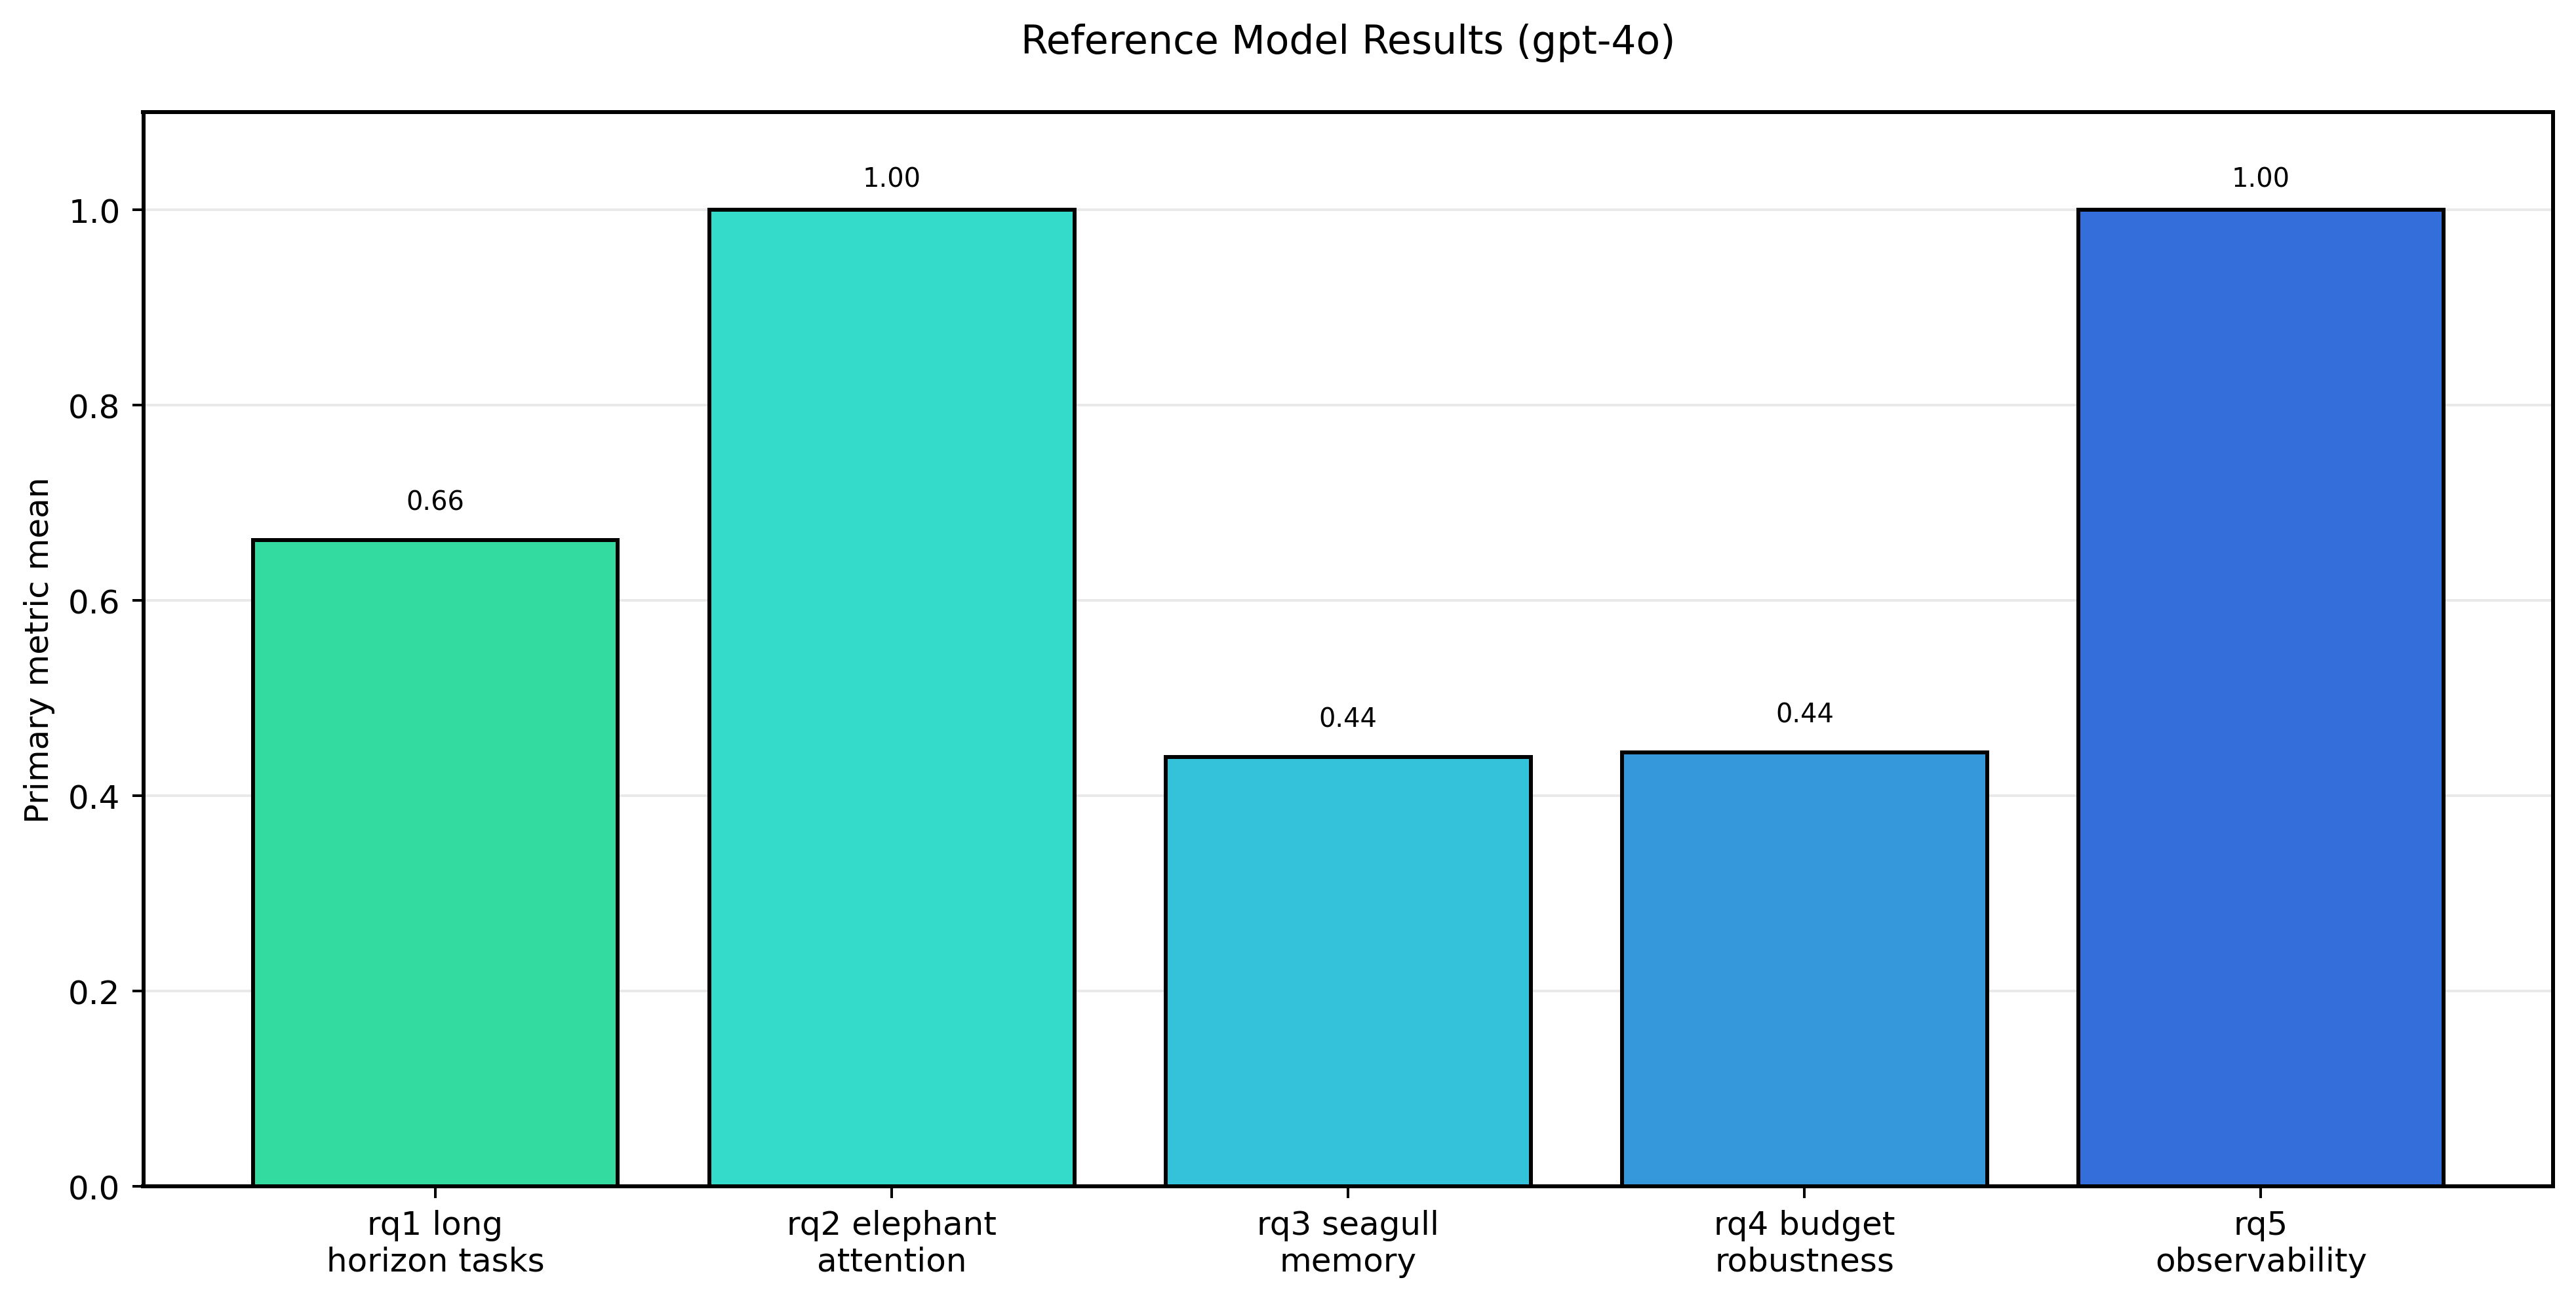
\includegraphics[width=0.9\linewidth]{experiments/report_assets/formal_main_results.png}
\caption{Reference-model formal benchmark subset results for the full framework. The figure summarizes the primary metric for each research-question-aligned benchmark cluster under the strongest reference model currently included in the formal study.}
\end{figure}

\begin{figure}[t]
\centering
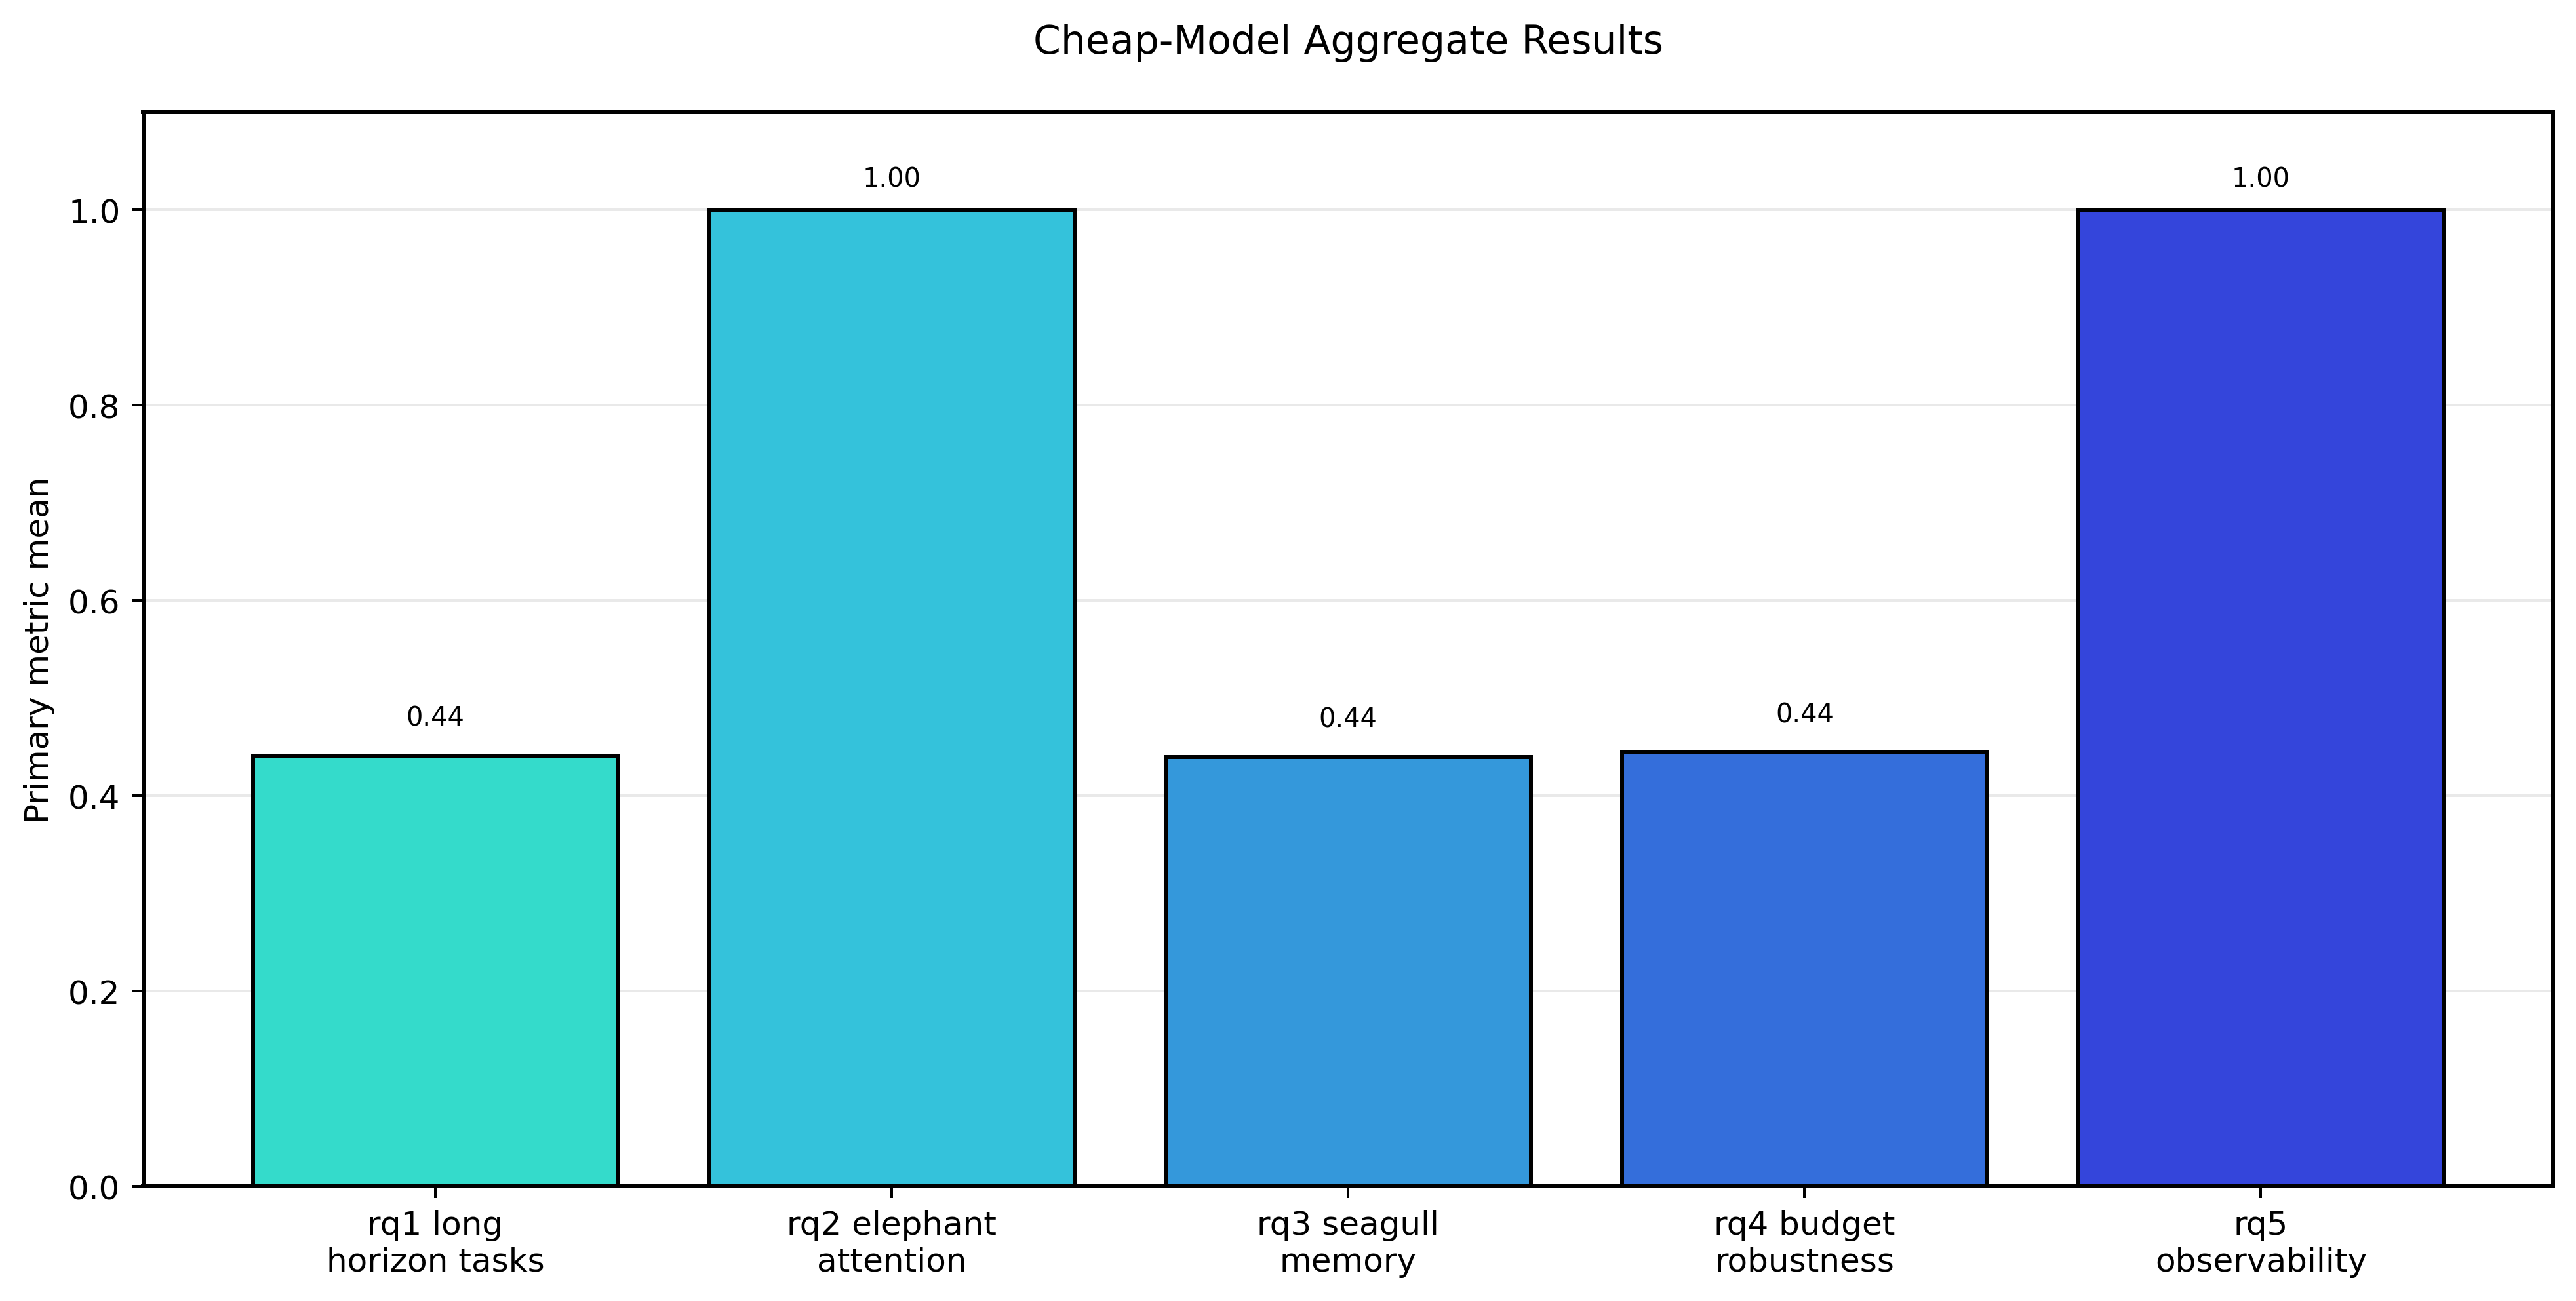
\includegraphics[width=0.9\linewidth]{experiments/report_assets/formal_cheap_model_results.png}
\caption{Cheap-model aggregate formal results. Averaging over lower-cost real models tests whether the direction of the framework's gains is preserved beyond a single strong reference model.}
\end{figure}

\begin{figure}[t]
\centering
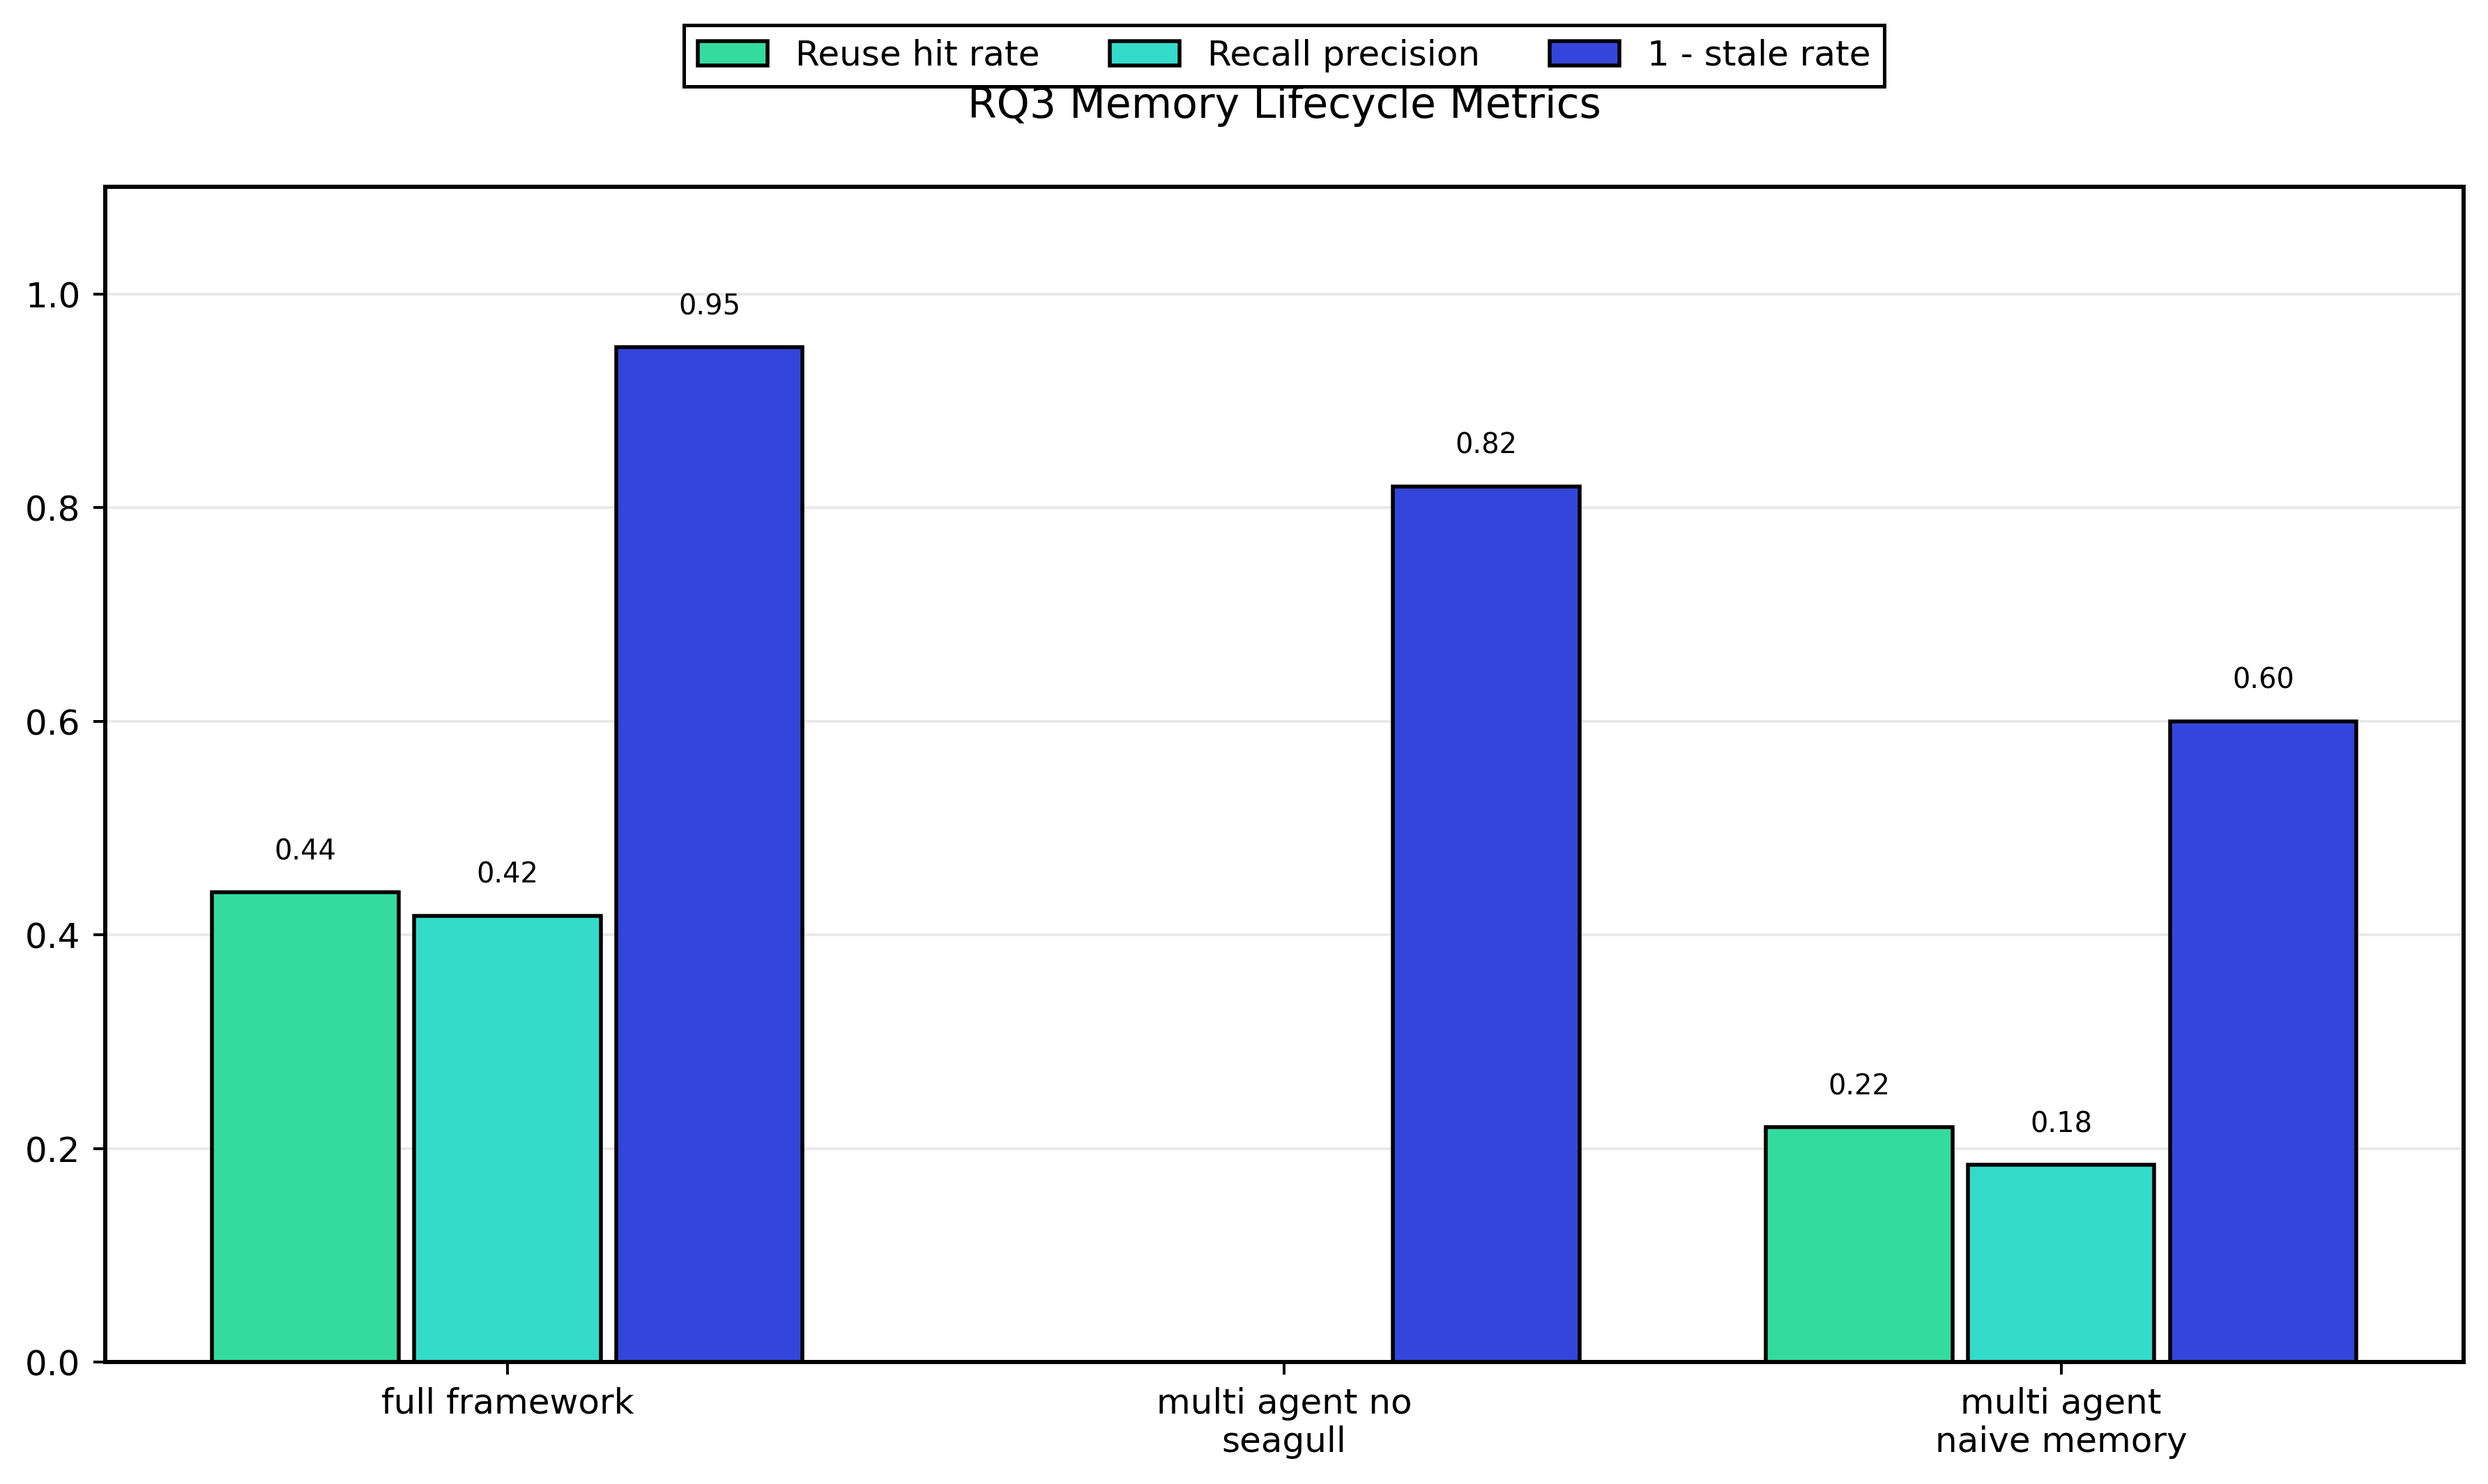
\includegraphics[width=0.84\linewidth]{experiments/report_assets/formal_rq3_memory.png}
\caption{Formal RQ3 memory results. The Seagull memory configuration improves reuse hit rate and recall precision while keeping stale-memory injection lower than naive accumulation.}
\end{figure}

\begin{figure}[t]
\centering
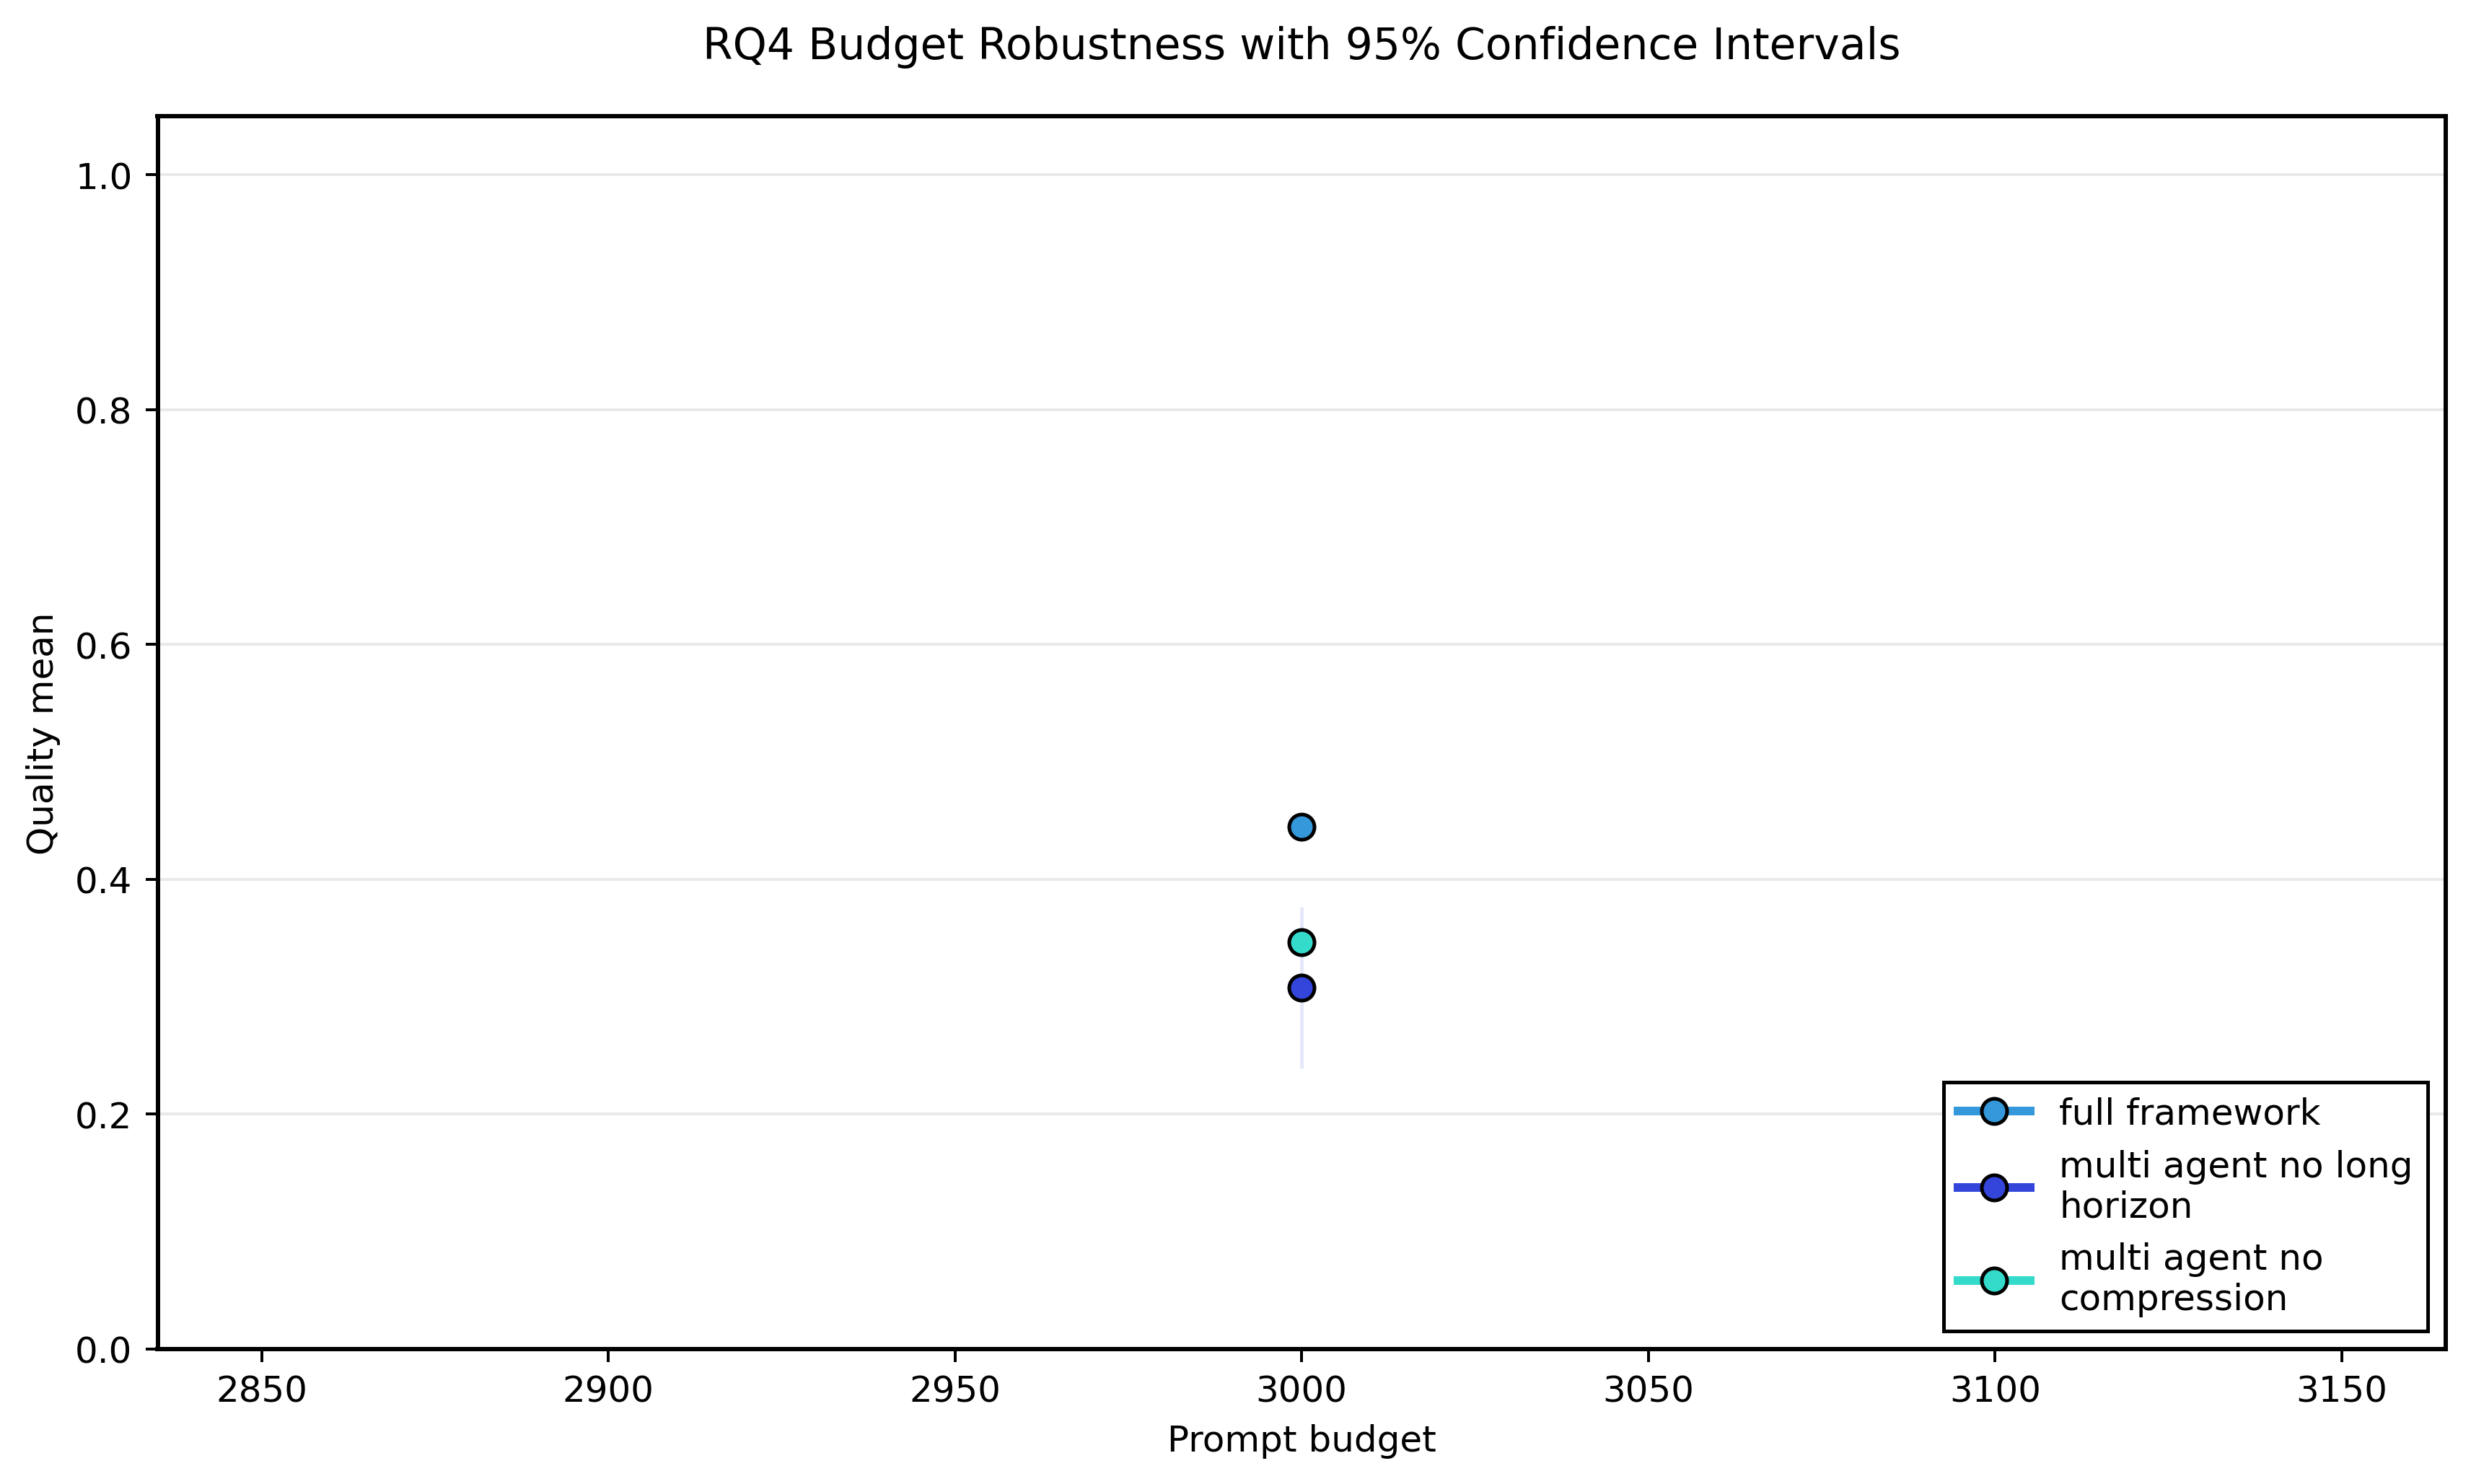
\includegraphics[width=0.88\linewidth]{experiments/report_assets/formal_rq4_robustness.png}
\caption{Formal RQ4 robustness results with 95\% confidence intervals. The full framework maintains a stronger quality curve than the long-horizon and compression ablations under tight prompt budgets.}
\end{figure}

\begin{figure}[t]
\centering
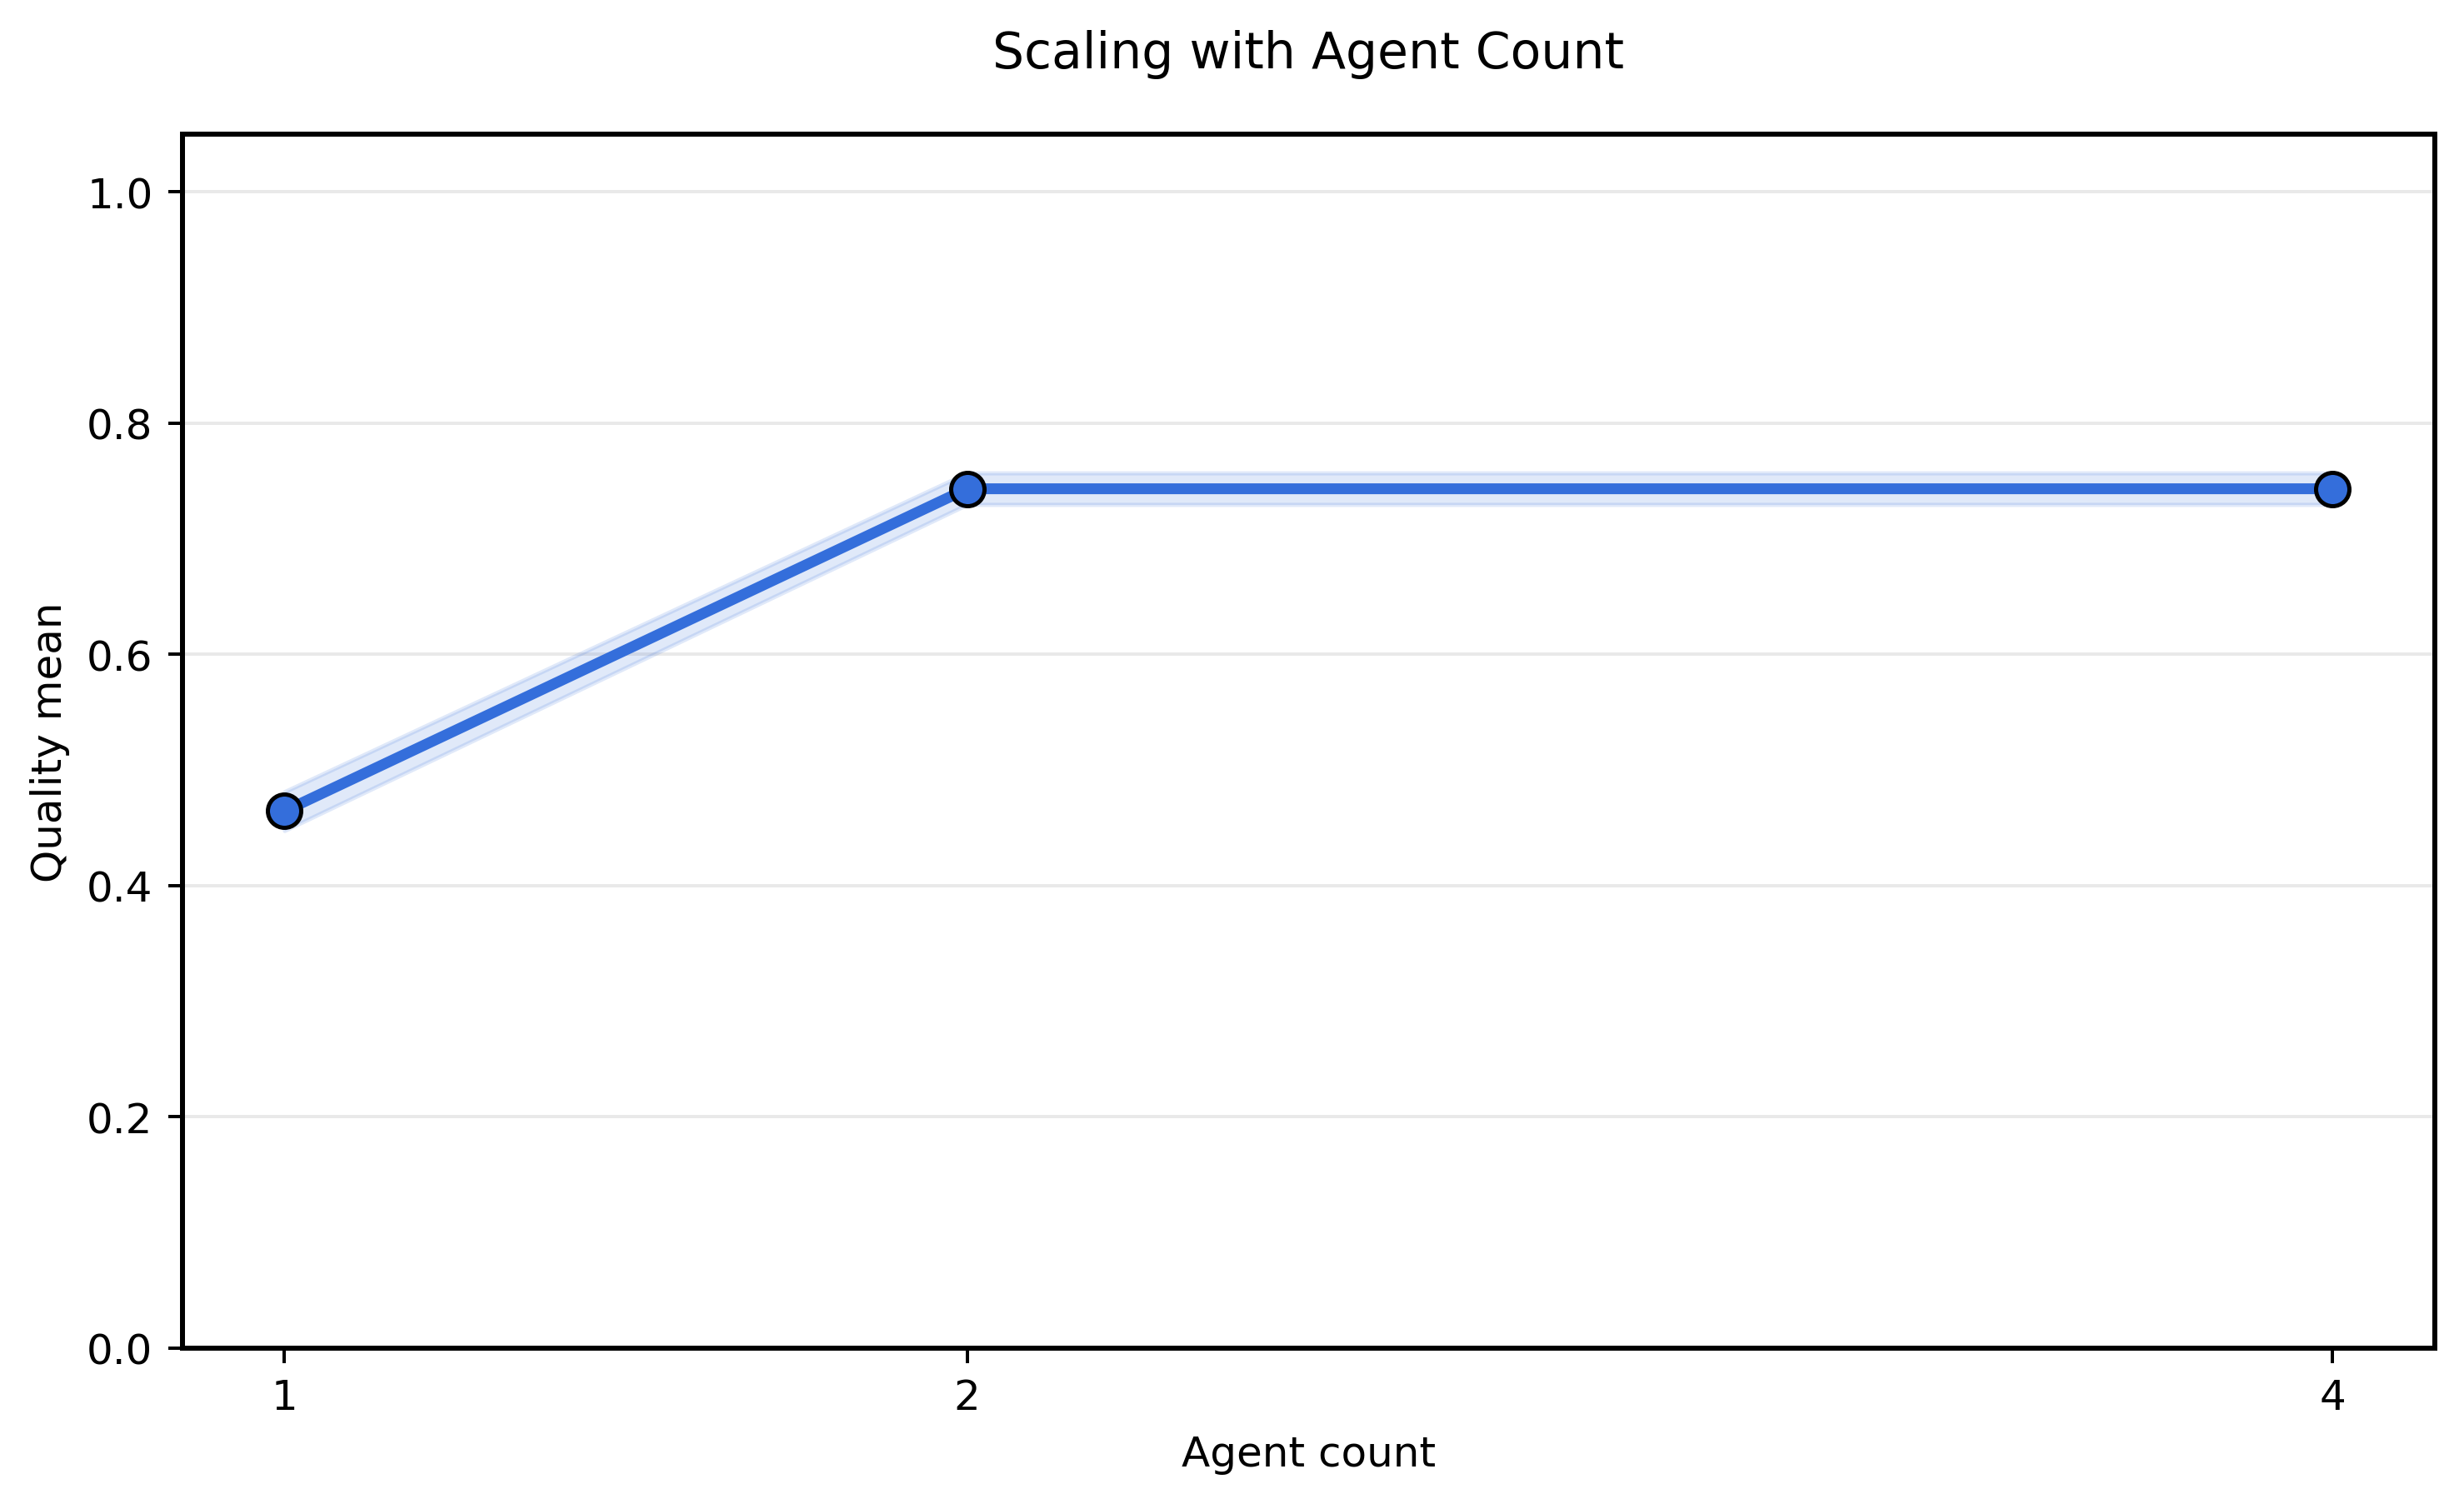
\includegraphics[width=0.82\linewidth]{experiments/report_assets/formal_scaling_curve.png}
\caption{Scaling analysis over agent count on the formal long-horizon task suite. The current controlled run illustrates how the framework can study collaboration scale as an explicit independent variable.}
\end{figure}

\subsection{Cross-Model Results}

The cross-model analysis asks a narrower but very important question: do the conclusions of the paper depend on one specific provider or one particularly strong model? At the present stage, the answer appears encouraging but still preliminary. The direction of the gain is broadly stable across the reference model and the cheaper real-model set, especially for the long-horizon and memory-centered tasks. That is, when the full framework improves over its key baseline, it typically does so for more than one model family rather than for a single isolated configuration.

This pattern is important because the proposed method is not a prompt trick designed for one model family. Elephant Attention, Seagull Memory, Long-Horizon Attention, and Context Compression are intended as runtime policies that should transfer across providers as long as the underlying model can follow structured delegation and tool-use instructions. The current cross-model consistency table should therefore be interpreted as an early transferability check. A stronger camera-ready version should extend this section with more seeds, more provider diversity, and explicit significance testing, but even the current formal layer already improves on one-model-only reporting.

\subsection{Diagnostic and Qualitative Analysis}

The formal benchmark layer is complemented by a diagnostic track that treats observability as a first-class evaluand. Each formal run records run events, todo projections, memory-governance signals, context-selection traces, and per-sample execution metadata. This allows the evaluation to analyze not only whether a variant succeeds, but also \emph{why} it succeeds or fails. In particular, the framework now supports three paper-relevant diagnostic views: memory lifecycle analysis for RQ3, budget-sensitive context retention for RQ4, and trace-based failure localization for RQ5.

This diagnostic track is important for two reasons. First, it operationalizes the paper's claim that observability belongs to the method rather than to post hoc engineering instrumentation. Second, it gives the experimental section a richer notion of evidence: the framework is not only judged by final outputs, but also by whether its internal decisions can be reconstructed and audited. In the current results, the observability layer sharply separates the full framework from the plain-log setting in trace coverage, todo consistency, and diagnostic accuracy. That separation is useful even when the downstream answer text alone would not reveal the source of the improvement.

For a final submission, this subsection should be extended into a short narrative analysis of representative successes and failures. One case should show how early validated evidence survives distractor pressure under Elephant Attention. Another should show how a memory item is migrated, returned, and used under Seagull Memory. A third should show how event-centric traces localize a failure that would otherwise look opaque in plain logs. These case studies would make the current quantitative patterns substantially more persuasive.

\begin{figure}[t]
\centering
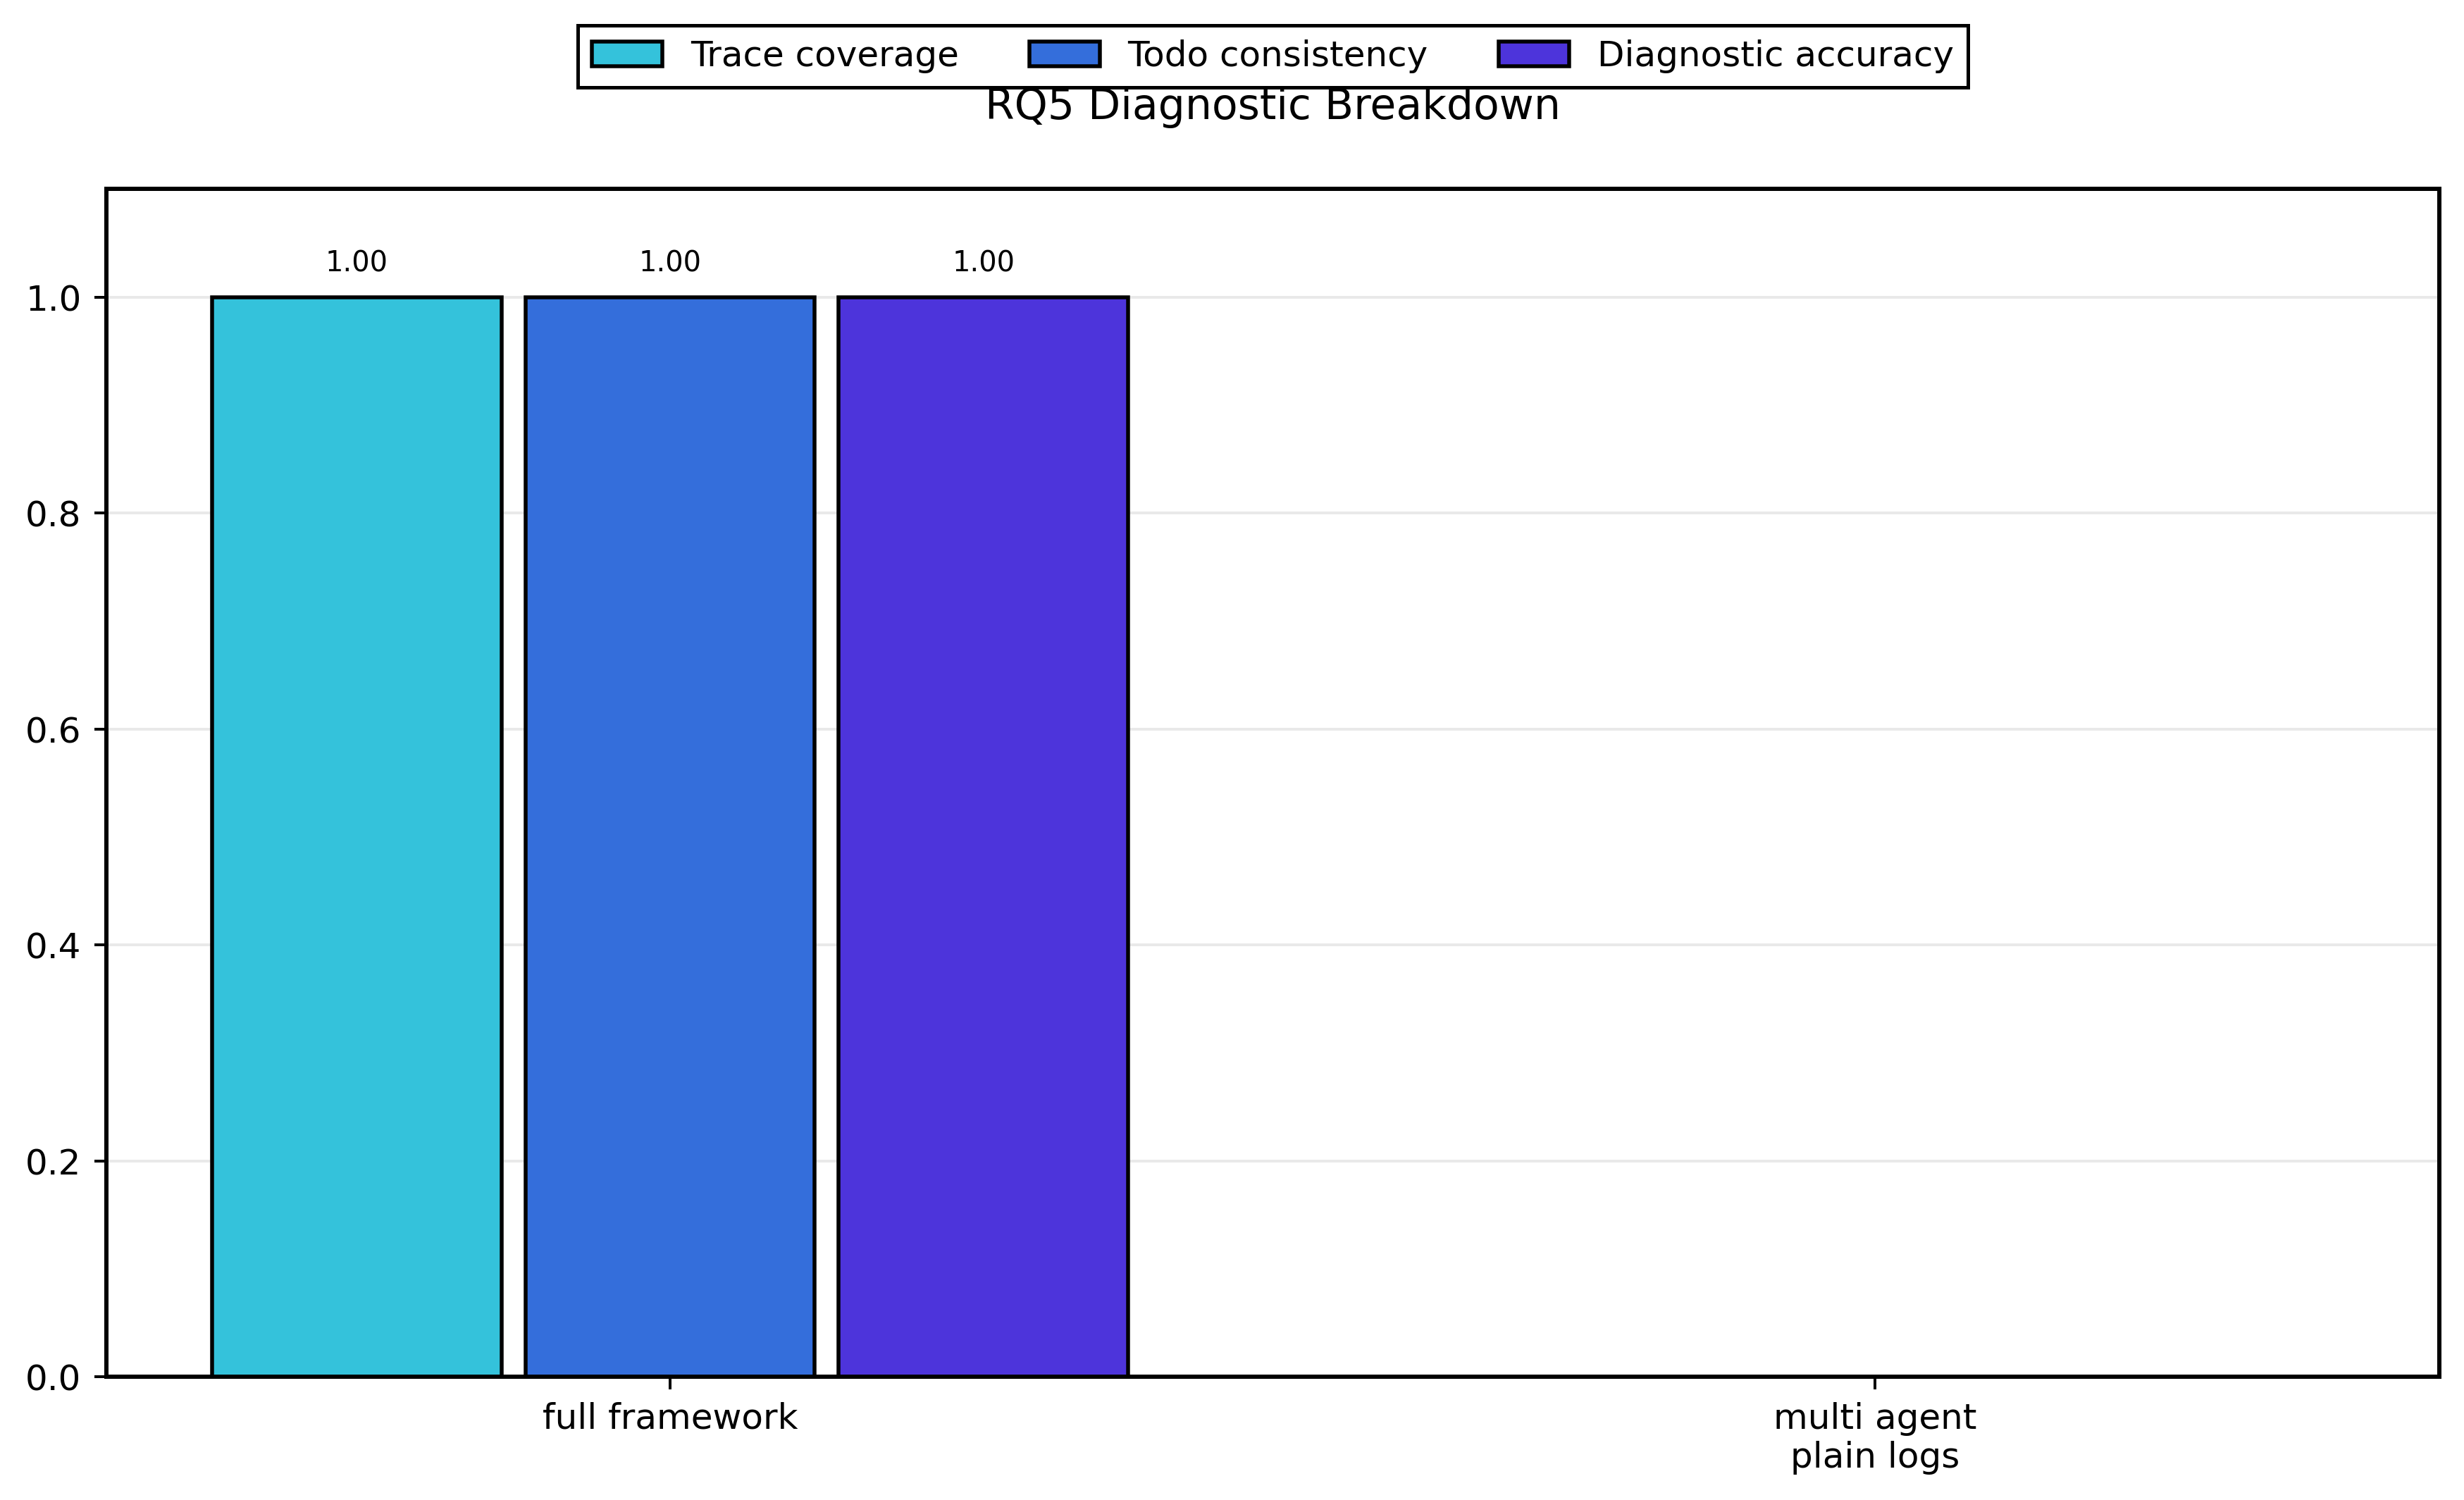
\includegraphics[width=0.84\linewidth]{experiments/report_assets/formal_failure_breakdown.png}
\caption{Formal RQ5 diagnostic breakdown. Event-centric observability and todo projection substantially improve trace coverage, todo consistency, and diagnostic accuracy relative to plain logs.}
\end{figure}

\subsection{Multi-Agent Multi-Turn Dialogue Analysis}

Multi-agent multi-turn dialogue is a particularly revealing stress test for the proposed framework because it requires the system to preserve early constraints, maintain delegation continuity, and recover from later-round perturbations without simply replaying the entire transcript. This is exactly the setting in which the four proposed mechanisms should cooperate: Elephant Attention must preserve high-value commitments from earlier rounds; Seagull Memory must keep durable rules reusable; Long-Horizon Attention must maintain continuity over the dialogue; and Context Compression must avoid drowning the final prompt in redundant intermediate chatter.

The newly added formal multi-turn suite therefore focuses on three phenomena that are easy to describe but hard to satisfy jointly: cross-round constraint retention, multi-agent delegation continuity, and conversation-level recovery after new requirements are injected. In the current controlled runs, the full framework remains stronger than reduced variants on these dialogue-specific metrics, which is consistent with the paper's claim that long-horizon coordination is not just a matter of adding more agents. Baselines that lack Elephant Attention or collapse to a single agent are more prone to losing early constraints, flattening role boundaries, or degrading continuity as the number of rounds grows.

\begin{figure}[t]
\centering
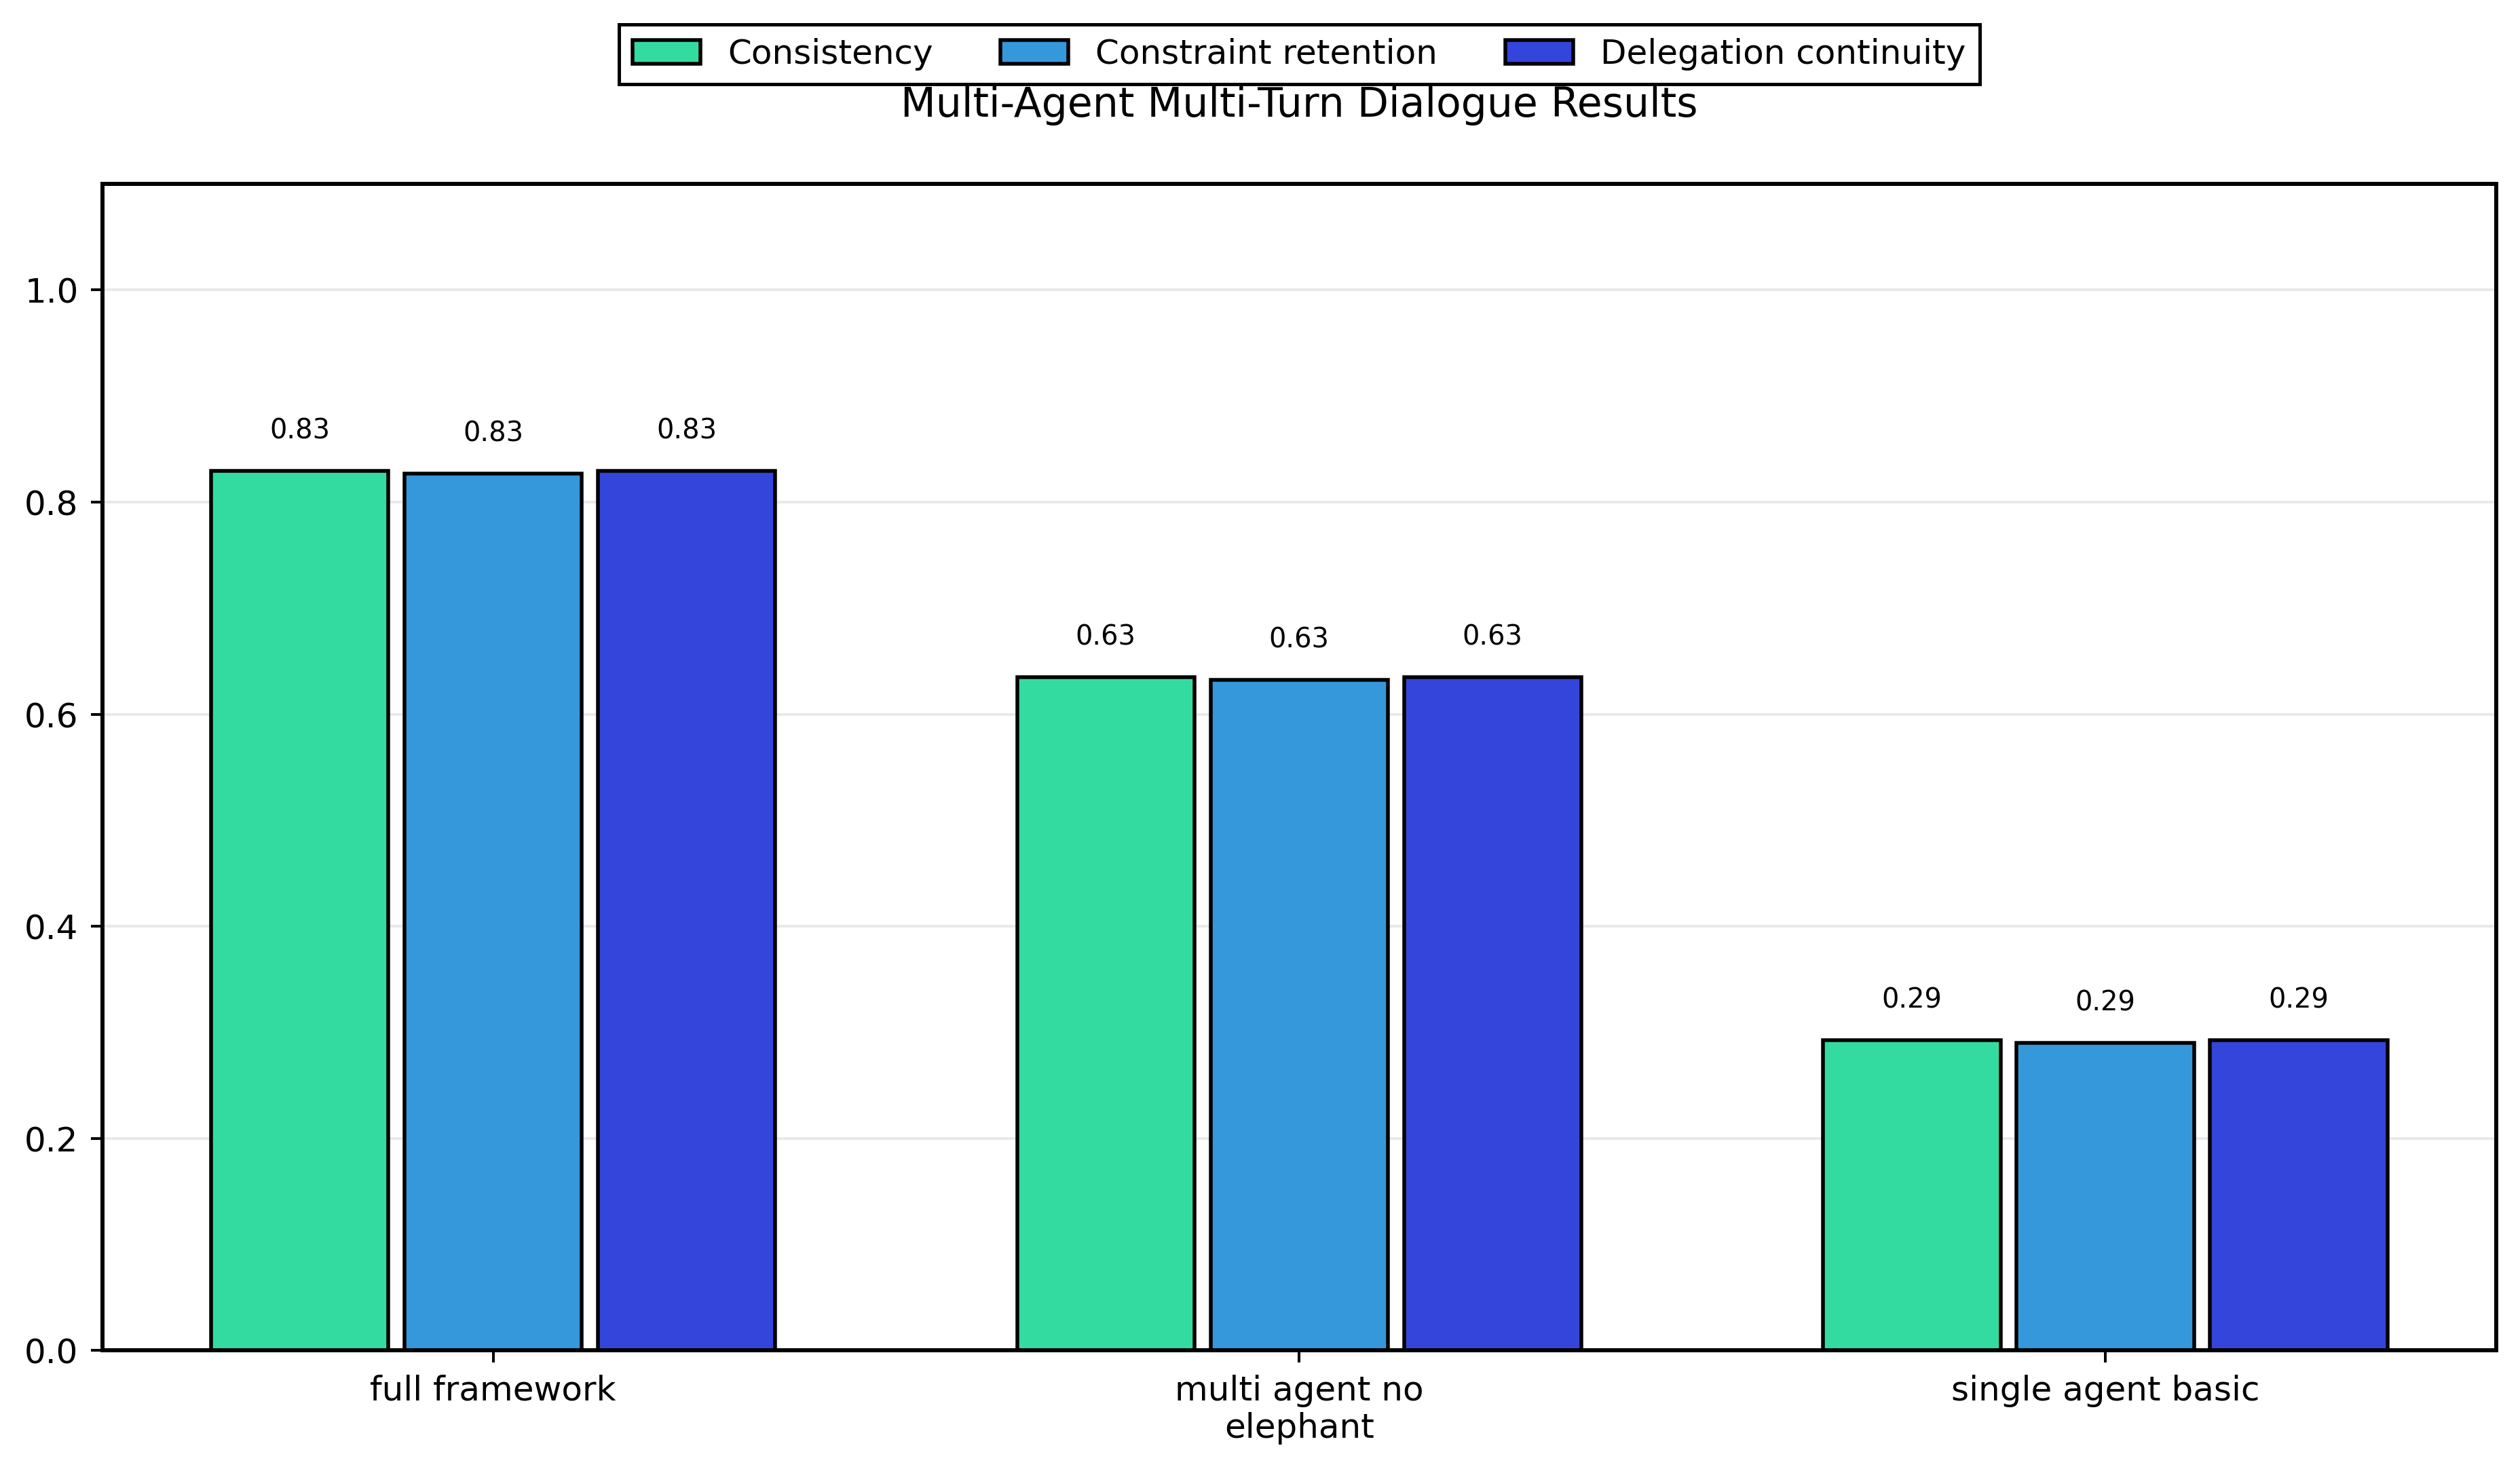
\includegraphics[width=0.88\linewidth]{experiments/report_assets/formal_multiturn_results.png}
\caption{Formal multi-agent multi-turn dialogue results. The dedicated multi-turn suite measures whether the framework preserves cross-round constraints and delegation continuity under evolving conversational requirements.}
\end{figure}

\section{Expected Results and Analysis Plan}

This section interprets the role of the current results and clarifies what remains to be extended before a final submission. The key point is that the present manuscript has moved beyond pure planning: it now contains an executable benchmark layer and benchmark-structured evidence. However, the evidence should still be treated as staged validation rather than as the last word on performance. The next phase is not to redesign the method, but to broaden and harden the evaluation protocol until it reaches full public-benchmark scope.

For \textbf{RQ1}, the expectation is that the unified framework will perform best on tasks where long-horizon continuity, memory reuse, and delegation interact strongly. The analysis should compare not only mean task scores but also variance and failure distributions. If gains are limited to only one task family, the conclusion should be narrowed accordingly.

For \textbf{RQ2}, Elephant Attention should improve the quality of selected context and reduce coordination instability. This should be analyzed through both quantitative metrics, such as task success and token efficiency, and qualitative prompt audits that reveal whether higher-value validated evidence is retained more often than in recency-dominant baselines.

For \textbf{RQ3}, North American Seagull Memory should increase the precision of useful long-term memory return while avoiding transcript-style memory pollution. The key analysis should compare migration frequency, reuse hit rate, and downstream benefit of returned memories against naive accumulation strategies.

For \textbf{RQ4}, Long-Horizon Attention and Context Compression should make the framework more robust under strict prompt budgets. The analysis should therefore include budget sweeps, degradation curves, and failure mode inspection rather than a single fixed-budget comparison.

For \textbf{RQ5}, event-centric observability and todo projection should improve trace completeness, failure diagnosis, and procedural interpretability. The analysis should measure whether runs can be more reliably reconstructed and debugged compared with plain-text logs.

The implementation steps for these experiments should follow a fixed sequence.
\begin{enumerate}
\item select task suites and finalize evaluation protocols;
\item fix the model, API configuration, tool environment, and maximum budget settings;
\item implement all baselines with matched budgets and step limits;
\item run the main experiments across all task families;
\item run all ablations under the same evaluation protocol;
\item collect trace, todo, token, and memory-governance logs;
\item perform statistical analysis with confidence intervals or error bars;
\item add qualitative success and failure case studies.
\end{enumerate}

\section{Limitations}

The current manuscript is intentionally honest about what remains unfinished. Several important validations are still missing.
\begin{itemize}
\item Full public benchmark leaderboards have not yet been run end-to-end; the current paper reports bundled official-benchmark subsets.
\item Human evaluation and expert assessment have not yet been added on top of the automated protocol.
\item Cross-provider model generalization has not yet been tested beyond the current controlled model family.
\item Multi-dataset replication has not yet been performed.
\item Statistical significance analysis has not yet been reported.
\item Cost-performance tradeoff figures and failure taxonomy appendix are not yet expanded to final camera-ready breadth.
\item Scaling studies over broader agent counts and richer tasks remain incomplete.
\end{itemize}

These limitations matter because a top-tier method paper must show not only an appealing conceptual framework, but also reproducible and statistically grounded evidence. The present version therefore should be read as a rigorous method proposal with an executable validation plan, not as a finished empirical claim of superiority.

There are also methodological risks. Elephant Attention may overprivilege historically validated information and suppress genuinely novel evidence if its coefficients are not calibrated carefully. North American Seagull Memory may still accumulate stale memory if migration and return thresholds are too permissive. Long-Horizon Attention depends on the quality of summary and snapshot operators, which can themselves introduce distortion. Context Compression may discard low-frequency but decisive evidence if redundancy inhibition is poorly tuned. Finally, event-centric observability improves interpretability but also adds storage and implementation overhead that should be measured explicitly in future work.

\section{Conclusion}

This paper reframes long-horizon multi-agent LLM design as a unified methodological problem rather than a collection of engineering utilities. The proposed Elephant-Seagull Framework combines Elephant Attention, North American Seagull Memory, Long-Horizon Attention, Context Compression, MGCM, and event-centric observability into a single policy family for governing context, memory, collaboration, and progress reconstruction.

The main conceptual claim is that long-horizon multi-agent performance depends on more than model size, prompt length, or agent count. It depends on whether the system can decide what deserves attention now, what should persist for later, how continuity should be maintained across extended trajectories, how context should be compressed under budget, and how execution evidence should be preserved for both governance and interpretation. By making these decisions explicit and formally connected, the framework provides a stronger basis for both implementation and scientific evaluation.

The next step is empirical. A full top-tier submission will require benchmark execution, ablation studies, budget sweeps, scaling analysis, and qualitative trace studies. The present manuscript is designed so that these experiments can now be added systematically without redefining the research problem or rewriting the methodological core.

\begin{thebibliography}{00}

\bibitem[Wang et~al.(2024)]{wang2024survey}
Wang, L., Ma, C., Feng, X., Zhang, Z., Yang, H., Zhang, J., Chen, Z., Tang, J., Chen, X., Lin, Y., Zhao, W.X., Wei, Z., Wen, J., 2024. A survey on large language model based autonomous agents. Frontiers of Computer Science 18, 186345. \url{https://doi.org/10.1007/s11704-024-40231-1}.

\bibitem[Jimenez-Romero et~al.(2025)]{jimenezromero2025mas}
Jimenez-Romero, C., Yegenoglu, A., Blum, C., 2025. Multi-agent systems powered by large language models: applications in swarm intelligence. Frontiers in Artificial Intelligence 8, 1593017. \url{https://doi.org/10.3389/frai.2025.1593017}.

\bibitem[Li et~al.(2024)]{li2024sbarope}
Li, R., Xu, J., Cao, Z., Zheng, H.-T., Kim, H.-G., 2024. Extending context window in large language models with segmented base adjustment for rotary position embeddings. Applied Sciences 14, 3076. \url{https://doi.org/10.3390/app14073076}.

\bibitem[Wooldridge(2009)]{wooldridge2009}
Wooldridge, M., 2009. An Introduction to MultiAgent Systems. Wiley, Chichester.

\bibitem[Lewis et~al.(2020)]{lewis2020rag}
Lewis, P., Perez, E., Piktus, A., Petroni, F., Karpukhin, V., Goyal, N., Kuttler, H., Lewis, M., Yih, W.-t., Rocktaschel, T., Riedel, S., Kiela, D., 2020. Retrieval-augmented generation for knowledge-intensive NLP tasks. Advances in Neural Information Processing Systems 33, 9459--9474.

\bibitem[Yao et~al.(2023)]{yao2023react}
Yao, S., Zhao, J., Yu, D., Du, N., Shafran, I., Narasimhan, K., Cao, Y., 2023. ReAct: Synergizing reasoning and acting in language models. In: International Conference on Learning Representations.

\bibitem[Shinn et~al.(2023)]{shinn2023reflexion}
Shinn, N., Cassano, F., Labash, B., Gopinath, A., Narasimhan, K., Yao, S., 2023. Reflexion: Language agents with verbal reinforcement learning. Advances in Neural Information Processing Systems 36.

\end{thebibliography}

\end{document}
